\Chapter{EXTRACTION DE TAXONOMIE}
\label{chap:te}

Introduction et présentation générale \ldots \hl{Note : j'attends d'avoir rédigé la revue de littérature pour écrire l'introduction, puisqe j'aurais probablement à présenter les enjeux de l'extraction de taxonomie dans ce chapitre là}


\section{Présentation générale}
\subsection{Énoncé du problème}
\label{sec:te-problem}
Soit $\KG \subseteq \Ent \times \Rel \times \Ent$ un graphe de connaissance. Pour une entité $e \in \Ent$, on dit que $e$ est de type $t$ si le triplet $(e, \texttt{rdf:type}, t)$ appartient à $\KG$. Dans la littérature, les types sont souvent appelés des \textit{classes} : ici, on préfère l'usage de \textit{type} pour éviter des conflits de notation avec les \textit{clusters}, qui seront introduits dans la section~\ref{subsec:te-clustering}. Notons qu'une entité peut avoir plusieurs types : ainsi, \dbr{Charles\_Baudelaire} est à la fois de type \dbo{Poet}, \dbo{Writer} et \dbo{Agent}.

On note $\cal{T}$ l'ensemble des types contenus dans le graphe. L'enjeu est de construire une taxonomie $T$ sur $\cal{T}$, c'est-à-dire un ensemble d'axiomes de subsumption $\{(t_i \sqsubset t_i')\}_{i=1, \ldots}$. Un axiome $t \sqsubset t'$ signifie que $t'$ est un type plus général que $t$, et donc que tout élément de type $t$ est aussi de type $t'$. Dans ce cas, on dit que $t$ est un \textit{sous-type} de $t'$, et que $t'$ est un \textit{supertype} de $t$.
Pour être valide, une taxonomie $T$ doit vérifier une structure d'arbre, c'est-à-dire respecter deux conditions : chaque type doit avoir au plus un supertype, et $T$ ne doit pas contenir de cycle, donc ne doit contenir aucune séquence $t_0, t_1, \ldots, t_k$ telle que $t_0 \sqsubset t_1 \sqsubset \ldots \sqsubset t_k \sqsubset t_0$.


L'objectif est d'extraire l'information taxonomique contenue dans la géométrie des plongements vectoriels du graphe. On suppose donc avoir accès à un jeu de données $\cal{D} = \{ (\mathbf{e_i}, t_i) \}_{i=1, \ldots, N}$, constitué de $N$ plongements vectoriels typés, c'est-à-dire de $N$ paires $(\bf{e_i}, t_i) \in \R^d \times \cal{T}$ où $\bf{e_i}$ représente le plongement vectoriel de l'entité $e_i$, et $t_i$ son type. 

% Pourquoi ? extraire l'information taxonomique contenue dans la géométrie des plongements vectoriels + éviter d'exploiter des co-occurrences présentes dans les données, qui peuvent être causées par le fait que l'on a eu accès à une taxonomie lors de la création du graphe.
% Relâcher cette contrainte : donne accès au graphe complet, et pas seulement aux embeddings + avoir accès aux co-occurences. Dans ce cas, beaucoup plus d'information = donne la possibilité d'extraire une taxonomie plus riche, cf chapitre suivant.

\subsection{Idée générale}

Dans le problème de l'extraction de taxonomie, on est amené à manipuler des données sur deux plans : le premier est celui des types (\dbo{Person}, \dbo{Athlete}, \dbo{Artist}, \ldots) reliés entre eux par des liens de subsumption (par exemple, $\dbo{Athlete} \sqsubset \dbo{Person}$); le second est celui des instances et des groupes d'instances, dans lequel on dispose de liens de proximité entre instances, grâce aux plongements vectoriels, et de liens d'inclusion entre groupes d'instances. Ces deux plans sont liés : les entités sont liées aux types par la relation \texttt{rdf:type}, ce qui permet de représenter un type dans l'espace des entités par l'ensemble des instances de ce type, et de traduire l'axiome $\dbo{Athlete} \sqsubset \dbo{Person}$ par une relation d'inclusion entre les instances de \dbo{Athlete} et celles de \dbo{Person}. En pratique, cette liaison est imparfaite : il y a des entités dont les types sont inconnus, erronés ou arbitraires.

%entités qui possèdent ce type, et donc de traduire l'axiome 
%le pendant dans le plan des instances de l'axiome $\dbo{Athlete} \sqsubset \dbo{Person}$ est l'affirmation «le groupe des athlètes est inclus dans le groupe des personnes».

Si l'on dispose d'une taxonomie, on peut naturellement déduire une hiérarchie sur les groupes d'entités : ainsi, les entités de type \dbo{Agent} peuvent être divisées en deux sous-groupes, celui des \dbo{Organisation} et celui des \dbo{Person}; les entités de ce dernier groupe peuvent à leur tour être divisées en plusieurs sous-groupes (\dbo{Athlete}, \dbo{Artist}, etc.). Inversement, les plongements vectoriels d'entités fournissent un moyen pour créer une hiérarchie sur les groupes d'entités : il suffit pour cela d'appliquer un algorithme de regroupement hiérarchique sur ces plongements. Un tel algorithme regroupe les plongements en groupes, sur la base de leur proximité géométrique; on obtient une division des plongements en groupes géométriquement similaires, eux-même divisés en sous-groupes, et ainsi de suite. L'idée de notre méthode est d'utiliser cette hiérarchie sur les groupes pour induire une hiérarchie sur les types, autrement dit une taxonomie.

La section \ref{sec:te-method} décrit en détail la méthode proposée et ses deux variantes. La section \ref{sec:te-evaluation} évalue cette méthode et discute l'influence de chaque paramètre.

\section{Méthode proposée}
\label{sec:te-method}

\begin{figure}[h]
    \centering
    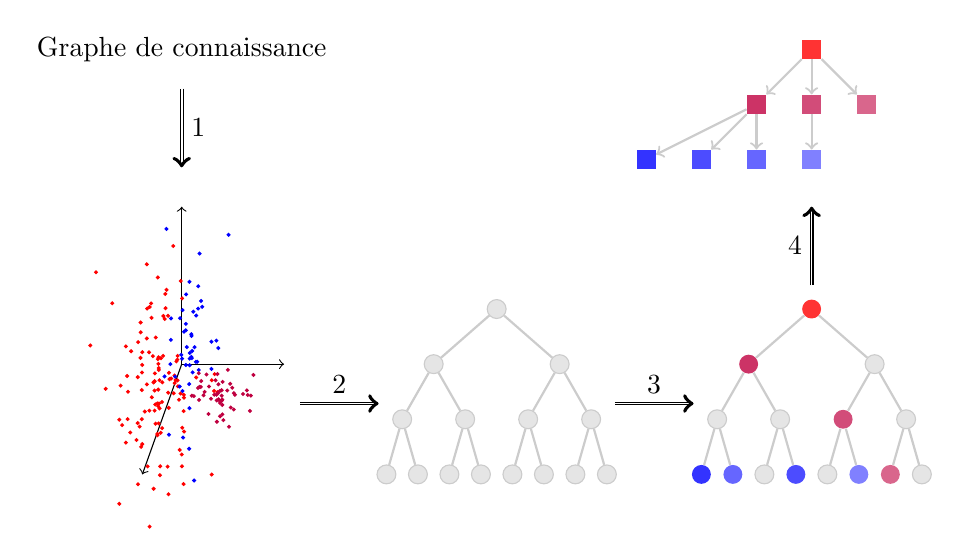
\begin{tikzpicture}
[   cnode/.style={draw=gray!40,fill=gray!20, minimum width=3mm, circle,inner sep=0.06, scale=0.8},
    colnode/.style={fill=#1,minimum width=3mm,circle,inner sep=0.06, scale=0.8},
    rnode/.style={draw=#1!40,fill=#1!20,minimum width=6mm, minimum height=6mm, rectangle},
    cline/.style={gray!40,thick},
    recnode/.style={fill=#1,minimum width=3mm, minimum height=3mm, rectangle, scale=0.8}
]

%
%\node at (0, 4.5) {Input Data};
\node at (0, 4) {Graphe de connaissance};
%\node at (0, 4) {$\{(e_i, t_i)\}$};

\draw [->] (0, 0) -- (0, 2);
\draw [->] (0, 0) -- (1.3, 0);
\draw [->] (0, 0) -- (-0.5, -1.4);

\draw [red] plot [only marks, draw=red, mark=*, mark size=0.5, domain=0:2, samples=120] ({2*(rnd-0.5)*rnd-0.3},{4*(rnd-0.5)*rnd-0.2});

\draw [blue] plot [only marks, draw=red, mark=*, mark size=0.5, domain=0:2, samples=50] ({(rnd-0.5)*rnd+0.1},{4*(rnd-0.5)*rnd+0.1});

\draw [purple] plot [only marks, draw=red, mark=*, mark size=0.5, domain=0:2, samples=50] ({1*(rnd-0.5)*rnd+0.5},{1*(rnd-0.5)*rnd-0.4});

%\node [red] at (-1.5, -1.5) {$t_1$};
%\node [blue] at (1.7, 1) {$t_2$};
%\node [purple] at (1.5, -1.5) {$t_3$};

    \draw[->, double] (0, 3.5) to[right] node {1} (0, 2.5);
    \draw[->, double] (1.5, -0.5) to[above] node {2} (2.5, -0.5);
    \draw[->, double] (5.5, -0.5) to[above] node {3} (6.5, -0.5);
    \draw[->, double] (8, 1) to[left] node {4} (8, 2); 

    % CLUSTERING %
    \def\offsetxa{4};
    \def\stepx{0.4};
    \def\stepy{0.7};
    
    \node[cnode] (000) at (-0.5*\stepx+\offsetxa,-2*\stepy) {};
    \node[cnode] (001) at (-1.5*\stepx+\offsetxa,-2*\stepy) {};
    \node[cnode] (010) at (-2.5*\stepx+\offsetxa,-2*\stepy) {};
    \node[cnode] (011) at (-3.5*\stepx+\offsetxa,-2*\stepy) {};
    \node[cnode] (100) at (0.5*\stepx+\offsetxa,-2*\stepy) {};
    \node[cnode] (101) at (1.5*\stepx+\offsetxa,-2*\stepy) {};
    \node[cnode] (110) at (2.5*\stepx+\offsetxa,-2*\stepy) {};
    \node[cnode] (111) at (3.5*\stepx+\offsetxa,-2*\stepy) {};
    
    \node[cnode] (00) at (-3*\stepx+\offsetxa,-\stepy) {};
    \node[cnode] (01) at (-1*\stepx+\offsetxa,-\stepy) {};
    \node[cnode] (10) at (1*\stepx+\offsetxa,-\stepy) {};
    \node[cnode] (11) at (3*\stepx+\offsetxa,-\stepy) {};
    
    \node[cnode] (0) at (-2*\stepx+\offsetxa,0*\stepy) {};
    \node[cnode] (1) at (2*\stepx+\offsetxa,0*\stepy) {};
    
    \node[cnode] (root) at (\offsetxa,\stepy) {};
    
    \draw[cline] (root) -- (0) {};
    \draw[cline] (root) -- (1) {};
    
    \draw[cline] (00) -- (0) {};
    \draw[cline] (10) -- (1) {};
    \draw[cline] (01) -- (0) {};
    \draw[cline] (11) -- (1) {};
    
    \draw[cline] (01) -- (000) {};
    \draw[cline] (01) -- (001) {};
    \draw[cline] (00) -- (010) {};
    \draw[cline] (00) -- (011) {};
    \draw[cline] (10) -- (100) {};
    \draw[cline] (10) -- (101) {};
    \draw[cline] (11) -- (110) {};
    \draw[cline] (11) -- (111) {};
    
    % CLUSTERING 2 %
    \def\offsetxc{\offsetxa+4};
    \def\stepx{0.4};
    \def\stepy{0.7};
    
    \node[colnode=blue!70] (000) at (-0.5*\stepx+\offsetxc,-2*\stepy) {};
    \node[cnode] (001) at (-1.5*\stepx+\offsetxc,-2*\stepy) {};
    \node[colnode=blue!60] (010) at (-2.5*\stepx+\offsetxc,-2*\stepy) {};
    \node[colnode=blue!80] (011) at (-3.5*\stepx+\offsetxc,-2*\stepy) {};
    \node[cnode] (100) at (0.5*\stepx+\offsetxc,-2*\stepy) {};
    \node[colnode=blue!50] (101) at (1.5*\stepx+\offsetxc,-2*\stepy) {};
    \node[colnode=purple!60] (110) at (2.5*\stepx+\offsetxc,-2*\stepy) {};
    \node[cnode] (111) at (3.5*\stepx+\offsetxc,-2*\stepy) {};
    
    \node[cnode] (00) at (-3*\stepx+\offsetxc,-\stepy) {};
    \node[cnode] (01) at (-1*\stepx+\offsetxc,-\stepy) {};
    \node[colnode=purple!70] (10) at (1*\stepx+\offsetxc,-\stepy) {};
    \node[cnode] (11) at (3*\stepx+\offsetxc,-\stepy) {};
    
    \node[colnode=purple!80] (0) at (-2*\stepx+\offsetxc,0*\stepy) {};
    \node[cnode] (1) at (2*\stepx+\offsetxc,0*\stepy) {};
    
    \node[colnode=red!80] (root) at (\offsetxc,\stepy) {};
    
    \draw[cline] (root) -- (0) {};
    \draw[cline] (root) -- (1) {};
    
    \draw[cline] (00) -- (0) {};
    \draw[cline] (10) -- (1) {};
    \draw[cline] (01) -- (0) {};
    \draw[cline] (11) -- (1) {};
    
    \draw[cline] (01) -- (000) {};
    \draw[cline] (01) -- (001) {};
    \draw[cline] (00) -- (010) {};
    \draw[cline] (00) -- (011) {};
    \draw[cline] (10) -- (100) {};
    \draw[cline] (10) -- (101) {};
    \draw[cline] (11) -- (110) {};
    \draw[cline] (11) -- (111) {};

%\node at (4, 0) {\Large $\Longrightarrow$};

% TAXONOMY
    \def\offsety{4};
    \def\offsetxtaxo{\offsetxc};

    \def\skipx{0.7};
    \def\skipy{0.7};
    
    \node[recnode=red!80] (l11) at (\offsetxtaxo, \offsety) {};
    
    \node[recnode=purple!80] (l21) at (-1*\skipx+\offsetxtaxo, \offsety-1*\skipy) {};
    \node[recnode=purple!70] (l22) at (\offsetxtaxo, \offsety-1*\skipy) {};
    \node[recnode=purple!60] (l23) at (1*\skipx+\offsetxtaxo, \offsety-1*\skipy) {};
    
    \node[recnode=blue!80] (l31) at (-3*\skipx+\offsetxtaxo, \offsety-2*\skipy) {};
    \node[recnode=blue!70] (l32) at (-2*\skipx+\offsetxtaxo, \offsety-2*\skipy) {};
    \node[recnode=blue!60] (l33) at (-1*\skipx+\offsetxtaxo, \offsety-2*\skipy) {};
    \node[recnode=blue!50] (l34) at (\offsetxtaxo, \offsety-2*\skipy) {};
    
    \draw[->, gray!40, thick] (l11) -- (l21) {};
    \draw[->, gray!40, thick] (l11) -- (l22) {};
    \draw[->, gray!40, thick] (l11) -- (l23) {};
    \draw[->, gray!40, thick] (l21) -- (l31) {};
    \draw[->, gray!40, thick] (l21) -- (l32) {};
    \draw[->, gray!40, thick] (l21) -- (l33) {};
    \draw[->, gray!40, thick] (l22) -- (l34) {};
\end{tikzpicture}
    \caption[Principe général de l'extraction de taxonomie]{Principe général de la méthode d'extraction de taxonomie : (1) les entités du graphe sont plongées dans un espace vectoriel, (2) ces plongements vectoriels sont regroupés hiérarchiquement, (3) les types des entités sont injectés dans la hiérarchie, puis finalement (4) l'association de la hiérarchie et des types est transformée en taxonomie.}
    \label{fig:te-summary}
\end{figure}

La méthode proposée ici se résume en trois étapes : d'abord, on effectue un regroupement hiérarchique des plongements vectoriels afin d'extraire un arbre de clustering, c'est-à-dire une hiérarchie sur les groupes d'entités (section \ref{subsec:te-clustering}); ensuite, les types des entités sont injectés dans cet arbre de clustering (section \ref{subsec:te-mapping}); enfin, une taxonomie est extraite en combinant les types et la structure d'arbre (section \ref{subsec:te-taxconstruction}). 

% création d'une hiérarchie sur des groupes d'entités à partir du regroupement hiérarchique de plongements vectoriels

% Une taxonomie est une hiérarchie sur des types, composée d'axiomes de subsumption $t \sqsubset t'$. Cette hiérarchie sur les types induit naturellement une hiérarchie sur des groupes d'entités : ainsi, les entités de type \dbo{Agent} peuvent être divisées en deux sous-groupes, celui des \dbo{Organisation} et celui des \dbo{Person}; les entités de ce dernier groupe peuvent à leur tour être divisées en plusieurs sous-groupes (\dbo{Athlete}, \dbo{Artist}, etc.). Or le regroupement hiérarchique appliqué aux plongements vectoriels d'entités permet justement d'obtenir une telle hiérarchie sur des groupes : cette méthode consiste à regrouper ensemble des points situés à proximité les uns des autres, puis à regrouper ces groupes entre eux, et ainsi de suite. Lorsqu'on l'applique à des plongements d'entités, on identifie donc des groupes d'entités géométriquement proches – donc sémantiquement similaires, ces groupes étant eux-mêmes subdivisés en sous-groupes, etc. Il reste alors à transformer cette hiérarchie sur des groupes d'entités en une hiérarchie sur les types eux-mêmes


% identifie des groupes d'entités géométriquement proches (donc sémantiquement proches), et subdivise ces groupes en sous-groupes

% Le préalable à notre méthode est le plongement du graphe dans $\R^d$. Pour cela, on s'appuie sur les travaux préliminaires décrits dans la section~\ref{chap:kge}. Notre point de départ est donc une matrice de dimension $N \times d$, qui peut être vue comme un nuage de points dans $\R^d$.

\subsection{Regroupement hiérarchique}
\label{subsec:te-clustering}

La première étape consiste à exécuter un algorithme de regroupement (ou \textit{clustering}) hiérarchique ascendant sur les plongements vectoriels des entités du jeu de données $\cal{D}$. %ce nuage de points. 
On commence avec $N$ groupes (ou \textit{clusters}) singletons, chacun contenant l'une des $N$ entités de départ. À chaque étape, deux des clusters existants sont fusionnés pour former un nouveau cluster. Les clusters à fusionner sont choisis de sorte à minimiser un certain critère : ce critère peut être la distance moyenne entre les entités des clusters, la distance minimale ou maximale entre ces entités, ou la variance du nouveau cluster. 
L'algorithme s'arrête lorsqu'il ne reste plus qu'un seul cluster qui contient toutes les entités; ce cluster est appelé cluster racine. Le résultat de cet algorithme est un arbre binaire, dont la racine est le cluster racine contenant toutes les entités, et dont les feuilles sont les $N$ clusters singletons. L'algorithme \ref{algo:te-clustering} contient le pseudo-code correspondant.

\begin{figure}[h]
    \centering
    \begin{adjustwidth}{0in}{-0.5in}
        \resizebox{1.1\textwidth}{!}{%
            \begin{tikzpicture}[
  arrow/.style={->, shorten >=3pt, gray!80},
  point/.style={circle,inner sep=0, minimum height=0.25cm, draw=#1, fill=#1, node distance=0.1cm},
  g1/.style={point=red},
  g2/.style={point=pink},
  g3/.style={point=purple},
  g4/.style={point=blue},
  g5/.style={point=cyan},
  cluster/.style={draw=gray, rounded corners=0.2cm},
  invisible/.style={inner sep=0}
]

\def\l{4}
\def\delta{0.2}
\def\sep{0.1}
\def\xmain{1}
\def\y{1}
\def\lstep{0.5cm}
\def\mid{0.05cm}


\foreach \pos [count=\i] in {0, 1, ..., 19}
    \node[invisible] (i0\i) at (\xmain*\pos, 0) {};

\node[anchor=south, below=\lstep of i01] {$\{e_1\}$};
\node[anchor=south, below=\lstep of i02] {$\{e_2\}$};
\node[anchor=south, below=0.7cm of i03] {$\ldots$};
\node[anchor=south, below=\lstep of i019] {$\{e_N \}$};

\foreach \pos [count=\i] in {0, 3, 5, 7, 9, 12, 14, 17}
    \node[invisible] (i1\i) at (\xmain*\pos+0.5*\xmain, \y) {};

\foreach \pos [count=\i] in {1, 6.5, 10, 15}
    \node[invisible] (i2\i) at (\xmain*\pos, 2*\y) {};
    
\foreach \pos [count=\i] in {4.5, 11.5, 16.5}
    \node[invisible] (i3\i) at (\xmain*\pos, 3*\y) {};
    
\foreach \pos [count=\i] in {2.5, 13.5}
    \node[invisible] (i4\i) at (\xmain*\pos, 4.5*\y) {};
    
\node[invisible] (i51) at (8.5*\xmain, 5.2*\y) {};



\draw[arrow, |->] (20*\xmain, 6.5*\y) to (20*\xmain, -\y);
\node[above] at (20*\xmain, 6.5*\y) {profondeur};
\foreach \yi [count=\i from 0] in {5.6, 4.3, 3, 2, 1, 0}{
    \draw (20*\xmain-0.1, \yi) -- (20*\xmain+0.1, \yi);
    \node[right] at (20*\xmain, \yi) {$\i$};
}
\foreach \col [count=\i] in {1, 1, 1, 2, 2, 3, 2, 3, 3, 4, 4, 4, 4, 4, 4, 1, 5, 5, 5}
{
    \node[g\col] (a0\i) at (i0\i) {};
    \node[cluster, fit=(a0\i) ] (c0\i) {};
 } 
 
\tikzset{bicluster/.style n args={3}{%
    g#1,
    left=\mid of i#3,
    append after command={\pgfextra{\let\main=\tikzlastnode}
        node[g#2, right=of \main] (a1#3) {} %
        node[cluster, fit=(\main)(a1#3)] (c#3) {} %
    }}
}

% \node[g1, left=\mid of i11] (a110) {};
% \node[g1, right=\mid of i11] (a111) {};
% \node[cluster, fit=(a110)(a111)] {};

\foreach \x/\y [count=\i] in {1/1, 2/2, 3/2, 3/3, 4/4, 4/4, 4/1, 5/5}
    \node[bicluster={\x}{\y}{1\i}] {};
    
\foreach \pos [count=\i] in {1, 4, 6, 8, 10, 13, 15, 18}
    {
    \draw[arrow] (c1\i) to (c0\pos);
}
\foreach \pos [count=\i] in {2, 5, 7, 9, 11, 14, 16, 19}
    {
    \draw[arrow] (c1\i) to (c0\pos);
}
% Triclusters
\node[g1] (a211) at (i21) {};
\node[g1, left=of a211] (a210) {};
\node[g1, right=of a211] (a212) {};
\node[cluster, fit=(a210)(a211)(a212)] (c21) {};
\draw[arrow] (c21) to (c11);
\draw[arrow] (c21) to (c03);

\node[g2, left=\mid of i22] (a221) {};
\node[g3, left=of a221] (a220) {};
\node[g3, right=\mid of i22] (a222) {};
\node[g3, right=of a222] (a223) {};
\node[cluster, fit=(a220)(a221)(a222)(a223)] (c22) {};
\draw[arrow] (c22) to (c13);
\draw[arrow] (c22) to (c14);

\node[g4] (a231) at (i23) {};
\node[g4, left=of a231] (a230) {};
\node[g4, right=of a231] (a232) {};
\node[cluster, fit=(a230)(a231)(a232)] (c23) {};
\draw[arrow] (c23) to (c15);
\draw[arrow] (c23) to (c012);

\node[g1] (a241) at (i24) {};
\node[g4, left=of a241] (a240) {};
\node[g5, right=of a241] (a242) {};
\node[cluster, fit=(a240)(a241)(a242)] (c24) {};
\draw[arrow] (c24) to (c17);
\draw[arrow] (c24) to (c017);

\node[g3, above=\mid of i31] (a311) {};
\node[g3, left=of a311] (a310) {};
\node[g2, right=of a311] (a312) {};
\node[g3, below=of a310] (a313) {};
\node[g2, right=of a313] (a314) {};
\node[g2, right=of a314] (a315) {};
\node[cluster, fit=(a310)(a311)(a312)(a313)(a314)(a315)] (c31) {};
\draw[arrow] (c31) to (c22) {};
\draw[arrow] (c31) to (c12) {};

\node[g4, above=\mid of i32] (a320) {};
\node[g4, left=of a320] (a321) {};
\node[g4, right=of a320] (a322) {};
\node[g4, below right=\mid and \mid of i32] (a323) {};
\node[g4, below left=\mid and \mid of i32] (a324) {};
\node[cluster, fit=(a320)(a321)(a322)(a323)(a324)] (c32) {};
\draw[arrow] (c32) to (c23);
\draw[arrow] (c32) to (c16);

\node[g1, above=\mid of i33] (a330) {};
\node[g4, left=of a330] (a331) {};
\node[g5, right=of a330] (a332) {};
\node[g5, below right=\mid and \mid of i33] (a333) {};
\node[g5, below left=\mid and \mid of i33] (a334) {};
\node[cluster, fit=(a330)(a331)(a332)(a333)(a334)] (c33) {};
\draw[arrow] (c33) to (c24);
\draw[arrow] (c33) to (c18);

\node[g3] (a410) at (i41) {};
\node[g1, above=of a410] (a411) {};
\node[g1, left=of a411] (a412) {};
\node[g1, right=of a411] (a413) {};
\node[g3, left=of a410] (a414) {};
\node[g2, right=of a410] (a415) {};
\node[g2, below=of a410] (a416) {};
\node[g3, left=of a416] (a417) {};
\node[g2, right=of a416] (a418) {};
\node[cluster, fit=(a410)(a412)(a418), label=115:{gauche(\texttt{racine})}] (c41) {};
\draw[arrow] (c41) to (c21);
\draw[arrow] (c41) to (c31);

\node[g4, left=\mid of i42] (a420) {};
\node[g4, right=of a420] (a421) {};
\node[g1, right=of a421] (a422) {};
\node[g4, left=of a420] (a423) {};
\node[g4, above=0.15cm of i42] (a424) {};
\node[g4, left=of a424] (a425) {};
\node[g4, right=of a424] (a426) {};
\node[g5, below=0.15cm of i42] (a427) {};
\node[g5, right=of a427] (a428) {};
\node[g5, left=of a427] (a429) {};
\node[cluster, fit=(a424)(a427)(a422)(a423), label=45:{droite(\texttt{racine})}] (c42) {};
\draw[arrow] (c42) to (c32);
\draw[arrow] (c42) to (c33);

\node[g5] (x1) at (i51) {};
\node[g5, right=of x1] (x2) {};
\node[g5, right=of x2] (x3) {};
\node[g1, left=of x1] (x4) {};
\node[g4, left=of x4] (x5) {};
\foreach \i in {1, 2, ..., 5}
    \node[g4, above=of x\i] (y\i) {};
\foreach \i/\j in {1/3, 2/3, 3/3, 4/2, 5/2}
    \node[g\j, above=of y\i] (z\i) {};
\foreach \i in {1, 2, 3}
    \node[g1, above=of z\i] (w\i) {};
\node[g2, above=of z4] {};
\node[cluster, fit=(w3)(x5), label={$\texttt{racine} = \{ e_1, e_2, \ldots, e_N \}$}] (c51) {};
\draw[arrow] (c51) to (c41);
\draw[arrow] (c51) to (c42);
\end{tikzpicture}
        }%
    \end{adjustwidth}
    
    \caption[Principe du regroupement hiérarchique ascendant]{Exemple d'arbre de clustering obtenu par regroupement hiérarchique ascendant. La couleur des points représente leur étiquette $y_i$ et n'est pas utilisée lors du regroupement.}
    \label{fig:clustering_tree}
\end{figure}

\subsubsection{Notations}

On note $\Clusters$ l'ensemble des clusters, $X$ l'arbre de clustering obtenu, et $\texttt{racine}$ la racine de l'arbre – c'est-à-dire, le cluster contenant toutes les entités. On peut écrire $X = (V_X, E_X)$, avec $V_X = \Clusters$ l'ensemble des sommets de $X$, et $E_X = \{(C_i, C_i')\}_{i = 1, 2, \ldots } \subseteq \Clusters^2$ l'ensemble des arêtes de $X$.

Pour deux clusters $C$ et $C'$, on dit que $C$ est un \textit{prédécesseur} de $C'$ si $C$ appartient à l'unique chemin entre la racine et $C'$, et on a alors $C' \subseteq C$. Dans ce cas, on appelle $C'$ un \textit{successeur} de $C$. De plus, on dit que $C$ est un prédécesseur \textit{strict} de $C'$ si $C$ est un prédécesseur de $C'$ avec $C \neq C'$, auquel cas on a $C' \subset C$. La relation $\subset$ définit un ordre partiel sur l'arbre $X$.

Puisque $X$ est une hiérarchie sur les clusters, il vérifie la propriété suivante :
\begin{equation}
    \forall C_1, C_2 \in X, C_1 \cap C_2 \neq \emptyset \implies (C_1 \subseteq C_2 \lor C_2 \subseteq C_1)
\end{equation}
Dit autrement, deux clusters sont soit disjoints, soit inclus l'un dans l'autre.

Pour un cluster $C$ donné, on définit $X[C]$ le \textit{sous-arbre de racine $C$} comme l'arbre contenant $C$ et tous ses successeurs:
\begin{equation}
    X[C] = (\{C' \in X : C' \subseteq C\}, \{(C_1, C_2) \in E_X : C_2 \subset C_1 \subseteq C\})
\end{equation}

Enfin, on définit $\gauche(C)$ et $\droite(C)$ respectivement les sous-clusters gauche et droit de $C$, $\succs(C)$ l'ensemble des successeurs de $C$, et $\succs(C)^*$ l'ensemble des successeurs stricts de $C$.

\subsubsection{Critère de fusion}
\label{sec:te-clustering-linkage}

Plusieurs critères sont envisageables pour choisir les clusters à fusionner lors du regroupement. Ici, on en considère quatre : le saut minimum, le saut moyen, le saut maximum, et la distance de Ward. Chacun de ces critères suppose que l'on ait défini une distance $d$ entre les vecteurs à regrouper : cette distance peut être la distance euclidienne, la distance cosinus ou encore la distance de Manhattan. 

Notons $\cal{C}_t$ l'ensemble des clusters à l'étape $t$. Un critère de fusion est en réalité une distance $D$ entre les clusters, ou, vu autrement, un \textit{coût} de fusion; à chaque étape, on fusionne les clusters $A$ et $B$ qui ont la plus faible distance entre eux – autrement dit, on cherche à minimiser le coût de fusion tout au long de la construction de l'arbre. Ainsi, à l'étape $t$, on détermine les deux clusters à fusionner selon la formule :
\begin{equation}
    A_t, B_t = \argmin_{A, B \in \cal{C}_t} D(A, B)
\end{equation}
On crée alors un nouveau cluster $C_{t+1} = A_t \cup B_t$, et on retire les clusters $A_t$ et $B_t$; le nouvel ensemble de clusters s'écrit donc :
\begin{equation}
    \cal{C}_{t+1} = \{ A_t \cup B_t \} \cup \cal{C}_t \setminus \{ A_t, B_t \}
\end{equation}
Et on ajoute à l'arbre de clustering les arêtes $(A_t, C_{t+1})$ et $(B_t, C_{t+1})$.



\begin{algorithm}
\KwInput{un nuage de points $\{\bf{e}_1, \bf{e}_2, \ldots, \bf{e}_N$\}}
\KwOutput{un arbre de clustering $X$}
\Parameter{critère de fusion $D$}
$t \leftarrow  0$ \;
$\cal{C}_0 \leftarrow  \left\{ \{\bf{e}_1\}, \ldots, \{\bf{e}_N\} \right\}$\;
$X = (\cal{C}_0, \emptyset)$ \;

\While{ $| \cal{C}_t | > 1$}{
    \tcp{déterminer les clusters à fusionner}
    $A_t, B_t \leftarrow  \argmin_{A, B \in \cal{C}_t} D(A, B)$ \;
    $C_{t+1} \leftarrow  A_t \cup B_t$\;
    \tcp{mise à jour des clusters}
    $\cal{C}_{t+1} \leftarrow  \{ C_{t+1}  \} \cup \cal{C}_t \setminus \{ A_t, B_t \}$\;
    \tcp{mise à jour de l'arbre}
    $X \leftarrow (V_X \cup \{ C_{t+1} \}, E_X \cup \{ (A_t, C_{t+1} ), (B_t, C_{t+1} ) \})$\;
    $t \leftarrow t + 1$ \;
}
\Return{$X$}
\caption{Algorithme de regroupement hiérarchique ascendant}
\label{algo:te-clustering}
\end{algorithm}


On définit maintenant les quatres critères de fusion considérés dans la suite. 

\paragraph{Saut minimum}

La distance entre $A$ et $B$ est la distance \textit{minimale} entre un point de $A$ et un point de $B$ :
\begin{equation}
    D(A, B) = \min_{\bf{x} \in A, \bf{y} \in B} d(\bf{x}, \bf{y})
\end{equation}

\paragraph{Saut moyen}

Ici, la distance entre $A$ et $B$ est la distance \textit{moyenne} entre leurs entités :
\begin{equation}
    D(A, B) = \frac{1}{|A| \times |B|} \sum_{\bf{x} \in A} \sum_{\bf{y} \in B} d(\bf{x}, \bf{y})
\end{equation}

\paragraph{Saut maximum}

Cette fois, la distance entre $A$ et $B$ est la distance \textit{maximale} entre un point de $A$ et un point de $B$ :
\begin{equation}
    D(A, B) = \max_{\bf{x} \in A, \bf{y} \in B} d(\bf{x}, \bf{y})
\end{equation}

\paragraph{Distance de Ward}

Le critère de Ward consiste à minimiser l'augmentation d'inertie lors de la fusion de $A$ et de $B$. L'inertie d'un cluster $C$ est la somme des carrés des distances entre ses entités et son centroïde :
\begin{equation}
    I(C) = \sum_{\bf{x} \in C} \left[d\left(\bf{x}, g(C)\right)\right]^2
\end{equation}
Avec $g(C)$ le centroïde du cluster $C$, parfois appelé \textit{centre de gravité} et défini par :
\begin{equation}
    g(C) = \frac{1}{|C|} \sum_{\bf{y} \in C} \bf{y}
\end{equation}
L'augmentation d'inertie lors de la fusion de $A$ et de $B$ est égale à l'inertie de $A \cup B$, à laquelle on retranche l'inertie de $A$ et de $B$ (puisque ces deux clusters disparaissent lors de la fusion) :
\begin{align}
    \Delta I &= I(A \cup B) - I(A) - I(B) \nonumber \\
    &= \sum_{\bf{x} \in A\cup B} d(\bf{x}, g(A \cup B) )^2
    - \sum_{\bf{x} \in A} d(\bf{x}, g(A) )^2
    - \sum_{\bf{x} \in B} d(\bf{x}, g(B) )^2
    \label{eq:te-ward-1}
\end{align}

En pratique, lorsqu'on utilise le critère de Ward, on choisit d'utiliser la distance euclidienne $d_\text{euc}$, ce qui permet de réécrire l'équation \ref{eq:te-ward-1} de la façon suivante :
\begin{equation}
    \Delta I = \frac{|A| \times |B|}{|A| + |B|} \left\| g(A) - g(B) \right\|_2^2
\end{equation}
La preuve complète de ce résultat est laissée au lecteur; elle s'obtient en décomposant $\sum_{\bf{x} \in A\cup B} \|\bf{x} - g(A \cup B) \|_2^2$ en deux sommes $\sum_{\bf{x} \in A} \|(\bf{x} - g(A)) + (g(A) - g(A \cup B)) \|_2^2$ et $\sum_{\bf{x} \in B} \|(\bf{x} - g(B)) + (g(B) - g(A \cup B)) \|_2^2$, et en exprimant les distances à l'aide du produit scalaire usuel.

En stockant les centroïdes des clusters tout au long de l'algorithme, cette équation permet de calculer le coût de fusion de deux clusters sans devoir recalculer l'inertie de $I(A\cup B)$ à chaque étape. Ainsi, le coût de fusion pour le critère de Ward est finalement :
\begin{equation}
    D(A, B) = \frac{|A| \times |B|}{|A| + |B|} \left\| g(A) - g(B) \right\|_2^2
\end{equation}

% Considérations temportelles ? Complexité de l'algorithme ?
% Étape non-supervisée




\subsection{Association type-cluster}
\label{subsec:te-mapping}


Au terme du regroupement hiérarchique, on dispose d'un côté d'une hiérarchie sur des groupes d'entités (les clusters), et de l'autre une liste de types non hiérarchisée (les étiquettes du jeu de données). L'idée centrale de cette étape est d'utiliser la structure sur les entités pour créer une structure sur les types. Pour cela, on injecte les types dans l'arbre de clustering : soit en associant à chaque type un unique cluster, qui le représente au mieux; soit en associant à chaque type plusieurs clusters avec des scores d'association. Ces deux méthodes sont exposées dans les sections suivantes.


%On a d'un côté, une hiérarchie sur des groupes d'entités (les clusters), de l'autre, une liste de types non hiérarchisé; but de l'étape : fusionner ces deux sources d'information, utiliser la structure sur les entités pour créer une structure sur les types. Pour cela, on injecte les types dans l'arbre de clustering, en associant chaque type à un cluster. Pour ce faire, deux méthdoes : 
%- associer à chaque type un unique cluster
%- définir, pour chaque type, une probabilité d'injection, ou un score d'association avec tous les clusters


\subsubsection{Méthode 1: Association injective (\textit{Hard Mapping)}}
\label{ssubsec:te-hardmapping}

Pour pouvoir associer les types aux clusters pertinents, il faut mesurer à quel point un cluster $C$ donné représente un type $t$. Pour ce faire, on peut utiliser la précision et le rappel de ce cluster pour $t$. Posons $N_{C,t} = | e \in C, type(e) = t|$ le nombre d'entités de type $t$ contenues dans le cluster $C$,
$N_t = |e \in \mathcal{D}, type(e) = t|$ le nombre d'entités de type $t$ dans l'ensemble des données, et $N_C = | C |$ le nombre total d'entités dans le cluster $C$. On peut alors définir la précision, le rappel et la mesure $F_1$ :
\begin{align}
    p(t, C) &= \frac{N_{C, t}}{N_C} \\
    r(t, C) &= \frac{N_{C, t}}{N_t} \\
    F_1(t, C) &= 2 \cdot \frac{p(t, C)r(t, C)}{p(t, C) + r(t, C)} = 2 \cdot \frac{N_{C,t}}{N_C + N_t}
\end{align}

La mesure $F_1$ varie entre 0 et 1: 0 indique que le cluster $C$ ne contient aucune entité de type $t$; 1 signifie que le cluster contient uniquement des entités de type $t$ et que toutes les entités de type $t$ sont contenues dans le cluster. 

% Ideally, we would map type $t$ to the cluster that maximizes its F-score, \textit{i.e} choose $m^*(t) = \argmax_C F_1(C, t)$, but then we could have two types mapped to the same cluster. If two types $t_A$ and $t_B$ are mapped to the same cluster $C$, then any type that is mapped to a successor of $C$ will have both $t_A$ and $t_B$ as ancestors, and the resulting taxonomy will not be valid. The mapping thus need to be unambiguous. Formally, this condition means that we need to find a injective mapping between types and clusters $m^* : \mathcal{T} \rightarrow \mathcal{C}$, so that distinct types are mapped to distinct clusters.  

Idéalement, on souhaiterait associer chaque type $t$ au cluster qui maximise sa mesure $F_1$, et donc choisir $m^*(t) = \argmax_C F_1(t, C)$, mais on pourrait alors avoir deux types associés au même cluster. Or, si deux types $t_A$ et $t_B$ sont associés au même cluster $C$, alors tout type associé à un successeur de $C$ aurait à la fois $t_A$ et $t_B$ comme prédécesseurs, et la taxonomie résultante serait donc invalide, selon les conditions énoncées en section~\ref{sec:te-problem}. Il faut donc garantir une association univoque entre types et clusters. Formellement, cela signifie que la fonction d'association $m^* : \Types \rightarrow \Clusters$ entre les types et les clusters doit être injective :
\begin{equation}
    \forall t, t' \in \Types, t \neq t' \implies m^*(t) \neq m^*(t')
\end{equation}


Pour une injection $m : \Types \rightarrow \Clusters$, on définit un score $J(m)$ qui mesure la qualité de l'association type-cluster définie par $m$. Ce score est simplement la mesure $F_1$ globale induite par $m$ :
\begin{equation}
    J(m) = \sum_{t \in \mathcal{T}} F_1(t, m(t))
\end{equation}

Notre association optimale est alors :
\begin{equation}
    m^* = \argmax_{
\substack{m : \Types \rightarrow \Clusters \\ m\text{ injective}}} \sum_{t \in \mathcal{T}} F_1(t, m(t))
\label{eq:optim-mapping}
\end{equation}


L'équation~\ref{eq:optim-mapping} définit un problème d'affectation linéaire, pour lequel une solution optimale existe dans tous les cas (et est unique si les mesures $F_1$ sont uniques pour chaque cluster).
Cette solution optimale peut être trouvée par l'algorithme de Jonker-Volgenant, avec une complexité de $O(|\Clusters|^3)$ dans le pire des cas \cite{jonker1987shortest}. Toutefois, l'utilisation de l'heuristique \textit{Asymmetric Greedy Search} \cite{brown2017heuristic} permet de réduire cette complexité, tout en trouvant des solutions dont le score est supérieur à 99.9\% du score optimal, en moyenne.
%, which can be useful when the size of $\mathcal{D}$ increases.

\subsubsection{Méthode 2: Association multiple (\textit{Soft Mapping)}}
\label{ssubsec:te-softmapping}

L'approche précédente aboutit à une fonction de décision binaire : un axiome $(t_i \sqsubset t_j)$ est prédit ou non, sans intermédiaire possible. Ceci parce que la fonction $\argmax$ de l'équation~\ref{eq:optim-mapping} n'est pas continue. En conséquence, la taxonomie prédite est sensible à des légers changements dans les données d'entrée.

Dans cette version, on explore une version lissée de l'approche précédente : l'association entre types et clusters est conservée, mais elle est lissée en remplacant la fonction $\argmax$ par une fonction softmax. Ainsi, un type n'est plus associé à un unique cluster; on lui attribue plutôt un vecteur de probabilités qui, pour chaque cluster, mesure si ce cluster le représente  bien. Ensuite, comme précédemment, cette association type-cluster est utilisée pour transformer la hiérarchie des clusters en une hiérarchie des types. Par rapport au cas précédent, la condition d'injectivité de l'association disparaît : une étape supplémentaire est nécessaire pour transformer le graphe de subsumption en une taxonomie valide. Ainsi, la discontinuité identifiée précédemment ne disparaît pas, mais elle est déplacée : au lieu d'intervenir lors de l'extraction des axiomes de subsumption, elle apparaît lors de la création de la taxonomie prédite à partir de ces axiomes. 

% Dans le cas précédent, on cherchait à déterminer la position optimale $m^*(t)$ de chaque type $t$ dans l'arbre. Ici, on suppose

Comme précédemment, notre hypothèse est que chaque type $t$ est représenté par un cluster de l'arbre. Contrairement au cas précédent toutefois, on suppose que la localisation de ce cluster est entachée d'incertitude. Cette incertitude a plusieurs sources. Premièrement, l'arbre de clustering obtenu est imparfait (les clusters ne sont pas parfaitement homogènes) car les plongements vectoriels utilisés sont bruités. Ce bruit a lui-même plusieurs origines : en premier lieu, le graphe de connaissance initial est incomplet; certaines informations sont absentes, inconnues ou mal renseignées; ensuite, la procédure d'entraînement est stochastique, à la fois pour la génération des exemples négatifs $\Delta_-$ et pour la mise à jour des paramètres par descente de gradient; enfin, les modèles de plongement sont parfois incapables de représenter certaines situations du graphe (par exemple, les relations antisymétriques ne sont pas modélisées par DistMult). Deuxièmement, les types qui servent d'étiquettes aux entités peuvent contenir des erreurs ou des ambiguïtés. Par exemple, les classes \dbo{Politician} et \dbo{OfficeHolder} de DBpédia sont très proches, et l'attribution d'un type ou d'un autre à une entité est souvent arbitraire. Troisièmement, les données d'entrée sont tirées aléatoirement, et un seul de leur type est conservé dans le jeu d'entraînement. Ce tirage aléatoire peut lui aussi entraîner des fluctuations. Toutes ces raisons se cumulent et justifient de modéliser le cluster représentant un type $t$ par une \textit{variable aléatoire} $Z_t$, plutôt que de lui attribuer une valeur fixe $m(t)$ comme dans le cas précédent.

Formellement, on introduit une famille de variables aléatoires $\cal{Z} = (Z_t)_{t \in \Types}$, indépendantes et à valeur dans $\Clusters$. On interprète la variable $Z_t$ comme le cluster représentant $t$ parmi tous les clusters de l'arbre de clustering. Il nous faut attribuer une loi de probabilité à $Z_t$, c'est-à-dire quantifier la probabilité que le type $t$ soit représenté par un cluster $C$ donné. Pour cela, on transforme les mesures $F_1$ en probabilités, à l'aide d'une fonction softmax. Pour un type $t$ et un cluster $C$, on définit un score d'association $\sigma(t, C)$:
\begin{equation}
    \sigma(t, C) = \frac{\displaystyle e^{ \beta F_1(t, C)}}{\displaystyle \sum_{C' \in \mathcal{C}} e^{\beta F_1(t, C')}}
\end{equation}
Pour un type $t$ donné, la somme des scores d'association avec chaque cluster vaut 1, ce qui permet d'envisager ce score comme une probabilité :
\begin{equation}
    \forall t \in \cal{T}, \sum_{C \in \cal{C}} \sigma(t, C) = 1
\end{equation}
Le paramètre $\beta > 0$ contrôle la concentration de la distribution autour du maximum. Le cas $\beta \rightarrow 0$ attribue à tous les clusters la même probabilité, tandis que le cas $\beta \rightarrow \infty$ donne toute la masse de probabilité au cluster de $F_1$ maximum, ce qui se rapproche de l'approche précédente. Le choix de la valeur de $\beta$ est discuté dans la section \ref{sec:te-hp}.

On peut alors définir la loi de la variable aléatoire $Z_t$, en posant pour $C \in \Clusters$:
\begin{equation}
    P(Z_t = C) = \sigma(t, C)
\end{equation}
Par construction du softmax, la position la plus probable pour $Z_t$ est le cluster qui a la mesure $F_1$ la plus élevée; toutefois, des clusters qui ont une mesure $F_1$ proche de la valeur maximale se verront également attribuer des probabilités significatives. L'utilisation d'une exponentielle et un choix de $\beta \gg 1$ permet à l'inverse de faire approcher de zéro les valeurs de $F_1$ éloignées du maximum, et donc d'éviter les localisations aberrantes de $Z_t$. 


%\todo{Justifier l'indépendance}

On peut alors interpréter l'axiome $t' \sqsubset t$ comme un événement aléatoire, qui s'exprime en fonction des événements $(Z_t = C)$ et $(Z_{t'} = C)$, pour tous $C \in \Clusters$.
En effet, l'axiome $t' \sqsubset t$ signifie que les entités de type $t'$ sont également de type $t$, et donc que le cluster $Z_{t'}$ représentant $t'$ est un sous-cluster (immédiat ou non) de $Z_t$ le cluster représentant $t$, ce qui se traduit mathématiquement par la relation $(Z_{t'} \subset Z_{t})$.
Pour exprimer l'événement $(Z_{t'} \subset Z_{t})$, il suffit d'examiner les valeurs possibles de $Z_t$ et $Z_{t'}$, et de ne considérer que les cas ou l'un est inclus dans l'autre. On peut donc décomposer $(Z_{t'} \subset Z_{t})$  en union disjointe d'événements $(Z_t = C, Z_{t'} = C')$ pour toutes les paires de clusters $C, C'$ telles que $C' \subset C$ :
\begin{equation}
    (Z_{t'} \subset Z_{t}) = \bigsqcup_{\substack{C, C' \in \mathcal{C} \\ C' \subset C}} (Z_t = C, Z_{t'} = C')
\end{equation}
%
%correspond au cas où le cluster représentant $t'$ est un successeur du cluster représentant $t$.
%Une fois que l'on peut estimer la probabilité de l'événement $(Z_t = C)$, on peut également interpréter l'axiome $t' \sqsubset t$ comme un événément aléatoire. % En effet, on a dit en introduction que la relation de subsumption entre les types se traduisait par une relation d'inclusion entre des groupes d'entités;
%$t' \sqsubset t$ correspond au cas où le cluster représentant $t'$ est un successeur du cluster représentant $t$. 
%
En utilisant cette décomposition et l'indépendance des $Z_t$, on peut écrire :
% Dès lors, on peut interpréter l'événement $t' \sqsubset t$ comme l'événement $Z_t \prec Z_{t'}$, et donc, en utilisant l'indépendances des $Z_t$ : 
\begin{align}
    \label{eq:softmapping_2}
    P(t' \sqsubset t) &= P(Z_{t'} \subset Z_{t}) \\
    &= \sum_{\substack{C, C' \in \mathcal{C} \\ C' \subset C}} P(Z_{t }= C, Z_{t'} = C') \nonumber \\
    &= \sum_{\substack{C, C' \in \mathcal{C} \\ C' \subset C}} P(Z_{t }= C)\cdot P(Z_{t'} = C') \\
    &= \sum_{\substack{C, C' \in \mathcal{C} \\ C' \subset C}} \sigma(t, C) \cdot \sigma(t', C')
\end{align}
On obtient donc une formule qui attribue une probabilité à chaque axiome de subsumption en fonction des scores d'association type-cluster. Par rapport au cas précédent, la validité d'un axiome n'est plus évaluée de manière binaire, mais peut prendre n'importe quelle valeur entre 0 et 1. Cela permet, entre autres, plus de souplesse dans l'étape suivante de reconstruction de taxonomie : en éliminant les axiomes trop incertains, on minimise le nombre d'axiomes faux qui sont extraits, quitte à ne pas extraire certains axiomes vrais; inversement, en conservant des axiomes incertains, on extrait davantage d'axiomes, au risque d'extraire certains axiomes faux.

\begin{figure}[h]
    \centering
    \begin{tikzpicture}[
  box/.style={draw=gray, thick, align=center},
  arrow/.style={->, shorten >=3pt, gray!80},
  node/.style={draw=gray, fill=gray!20},
  hnode/.style={draw=accent1, fill=accent1!20},
  snode/.style={draw=accent1, fill=accent1!20, very thick},
  point/.style={circle, draw=gray!80, fill=gray!30, node distance=1cm and 0.5cm, inner sep=0, minimum height=0.25cm},
  spoint/.style={circle, draw=gray!80, fill=gray!30, node distance=1cm and 0.3cm, inner sep=0, minimum height=0.25cm},
  pointA/.style={fill=accent1, draw=accent1},
  pointB/.style={fill=accent2, draw=accent2},
]

\def\y{1.5cm};
\def\x{0.5cm};

\begin{scope}[xshift=-3cm]
\node[point, fill=accent1!60, label={[accent1]10:$0,3$}] (root) at (0, 0) {};
\node[point, below left=of root, fill=accent1!80, label={[accent1]130:$0,5$}] (a1) {};
\node[point, below right=of root] (a2) {};
\node[point, below left=of a1, fill=accent1!20, label={[accent1]180:$0,1$}] (b1) {};
\node[point, below left=of a2, fill=accent1!20, label={[accent1]0:$0,1$}] (b2) {};

% \node[point, below right=of a1] (b2) {};

\node[text=accent1, anchor=west] at (-2.75, 0.75cm) {Loi de $Z_A$};
\draw[draw=accent1] (-2.75cm, 1cm) rectangle (2cm, -3cm);

\draw[arrow] (root) to (a1);
\draw[arrow] (root) to (a2);
\draw[arrow] (a1) to (b1);
\draw[arrow] (a1) to (b2);
\end{scope}
%%%%%%%
% ZB
%%%%%%%%
\begin{scope}[xshift=3cm]
\node[point] (root) at (0, 0) {};
\node[point, below left=of root, fill=accent2!80, label={[accent2]130:$0,5$}] (a1) {};
\node[point, below right=of root, fill=accent2!60, label={[accent2]0:$0,3$}] (a2) {};
\node[point, below left=of a1] (b1) {};
\node[point, below left=of a2, fill=accent2!40, label={[accent2]0:$0,2$}] (b2) {};
% \node[point, below right=of a1] (b2) {};

\node[text=accent2, anchor=west] at (-2.75, 0.75cm) {Loi de $Z_B$};
\draw[draw=accent2] (-2.75cm, 1cm) rectangle (2cm, -3cm);

\draw[arrow] (root) to (a1);
\draw[arrow] (root) to (a2);
\draw[arrow] (a1) to (b1);
\draw[arrow] (a1) to (b2);
\end{scope}

\node at (0, -4cm) {$B \sqsubset A \iff Z_B \subset Z_A$ : 4 cas possibles};


\def\shift{1.5cm}
\def\shifty{-5cm}
\begin{scope}[yshift=\shifty, xshift=-3*\shift]
\node[spoint, pointA, label={[accent1]180:{$Z_A$}}] (root) at (0, 0) {};
\node[spoint, pointB, below left=of root, label={[accent2]180:{$Z_B$}}] (a1) {};
\node[spoint, below right=of root] (a2) {};
\node[spoint, below left=of a1] (b1) {};
\node[spoint, below left=of a2] (b3) {};
\node[spoint, below right=of a1] (b2) {};
\draw[arrow] (root) to (a1);
\draw[arrow] (root) to (a2);
\draw[arrow] (a1) to (b1);
\draw[arrow] (a1) to (b2);
\node[below=0.5cm of b2] (eq)  {\textcolor{accent1}{$0,3$} $\times$ \textcolor{accent2}{$0,5$}};
\node[right=0.3cm of eq] {$+$};
\end{scope}


\begin{scope}[yshift=\shifty, xshift=-\shift]
\node[spoint, pointA, label={[accent1]180:{$Z_A$}}] (root) at (0, 0) {};
\node[spoint, below left=of root] (a1) {};
\node[spoint, below right=of root] (a2) {};
\node[spoint, below left=of a1] (b1) {};
\node[spoint, below left=of a2] (b3) {};
\node[spoint, pointB, below right=of a1, label={[accent2]0:{$Z_B$}}] (b2) {};
\draw[arrow] (root) to (a1);
\draw[arrow] (root) to (a2);
\draw[arrow] (a1) to (b1);
\draw[arrow] (a1) to (b2);
\node[below=0.5cm of b2] (eq)  {\textcolor{accent1}{$0,3$} $\times$ \textcolor{accent2}{$0,2$}};
\node[right=0.3cm of eq] {$+$};
\end{scope}


\begin{scope}[yshift=\shifty, xshift=\shift]
\node[spoint, pointA, label={[accent1]180:{$Z_A$}}] (root) at (0, 0) {};
\node[spoint, below left=of root] (a1) {};
\node[spoint, pointB, below right=of root, label={[accent2]270:{$Z_B$}}] (a2) {};
\node[spoint, below left=of a1] (b1) {};
\node[spoint, below left=of a2] (b3) {};
\node[spoint, below right=of a1] (b2) {};
\draw[arrow] (root) to (a1);
\draw[arrow] (root) to (a2);
\draw[arrow] (a1) to (b1);
\draw[arrow] (a1) to (b2);
\node[below=0.5cm of b2] (eq)  {\textcolor{accent1}{$0,3$} $\times$ \textcolor{accent2}{$0,3$}};
\node[right=0.3cm of eq] {$+$};
\end{scope}


\begin{scope}[yshift=\shifty, xshift=3*\shift]
\node[spoint] (root) at (0, 0) {};
\node[spoint, pointA, below left=of root, label={[accent1]180:{$Z_A$}}] (a1) {};
\node[spoint, below right=of root] (a2) {};
\node[spoint, below left=of a1] (b1) {};
\node[spoint, below left=of a2] (b3) {};
\node[spoint, pointB, below right=of a1, label={[accent2]0:{$Z_B$}}] (b2) {};
\draw[arrow] (root) to (a1);
\draw[arrow] (root) to (a2);
\draw[arrow] (a1) to (b1);
\draw[arrow] (a1) to (b2);
\node[below=0.5cm of b2] (eq)  {\textcolor{accent1}{$0,5$} $\times$ \textcolor{accent2}{$0,2$}};
\end{scope}

\node[draw=black, inner sep=0.3cm] at (0, -9.5cm) {$P(B \sqsubset A) = P(Z_B \subset Z_A) = 0,4$};

\end{tikzpicture}
    %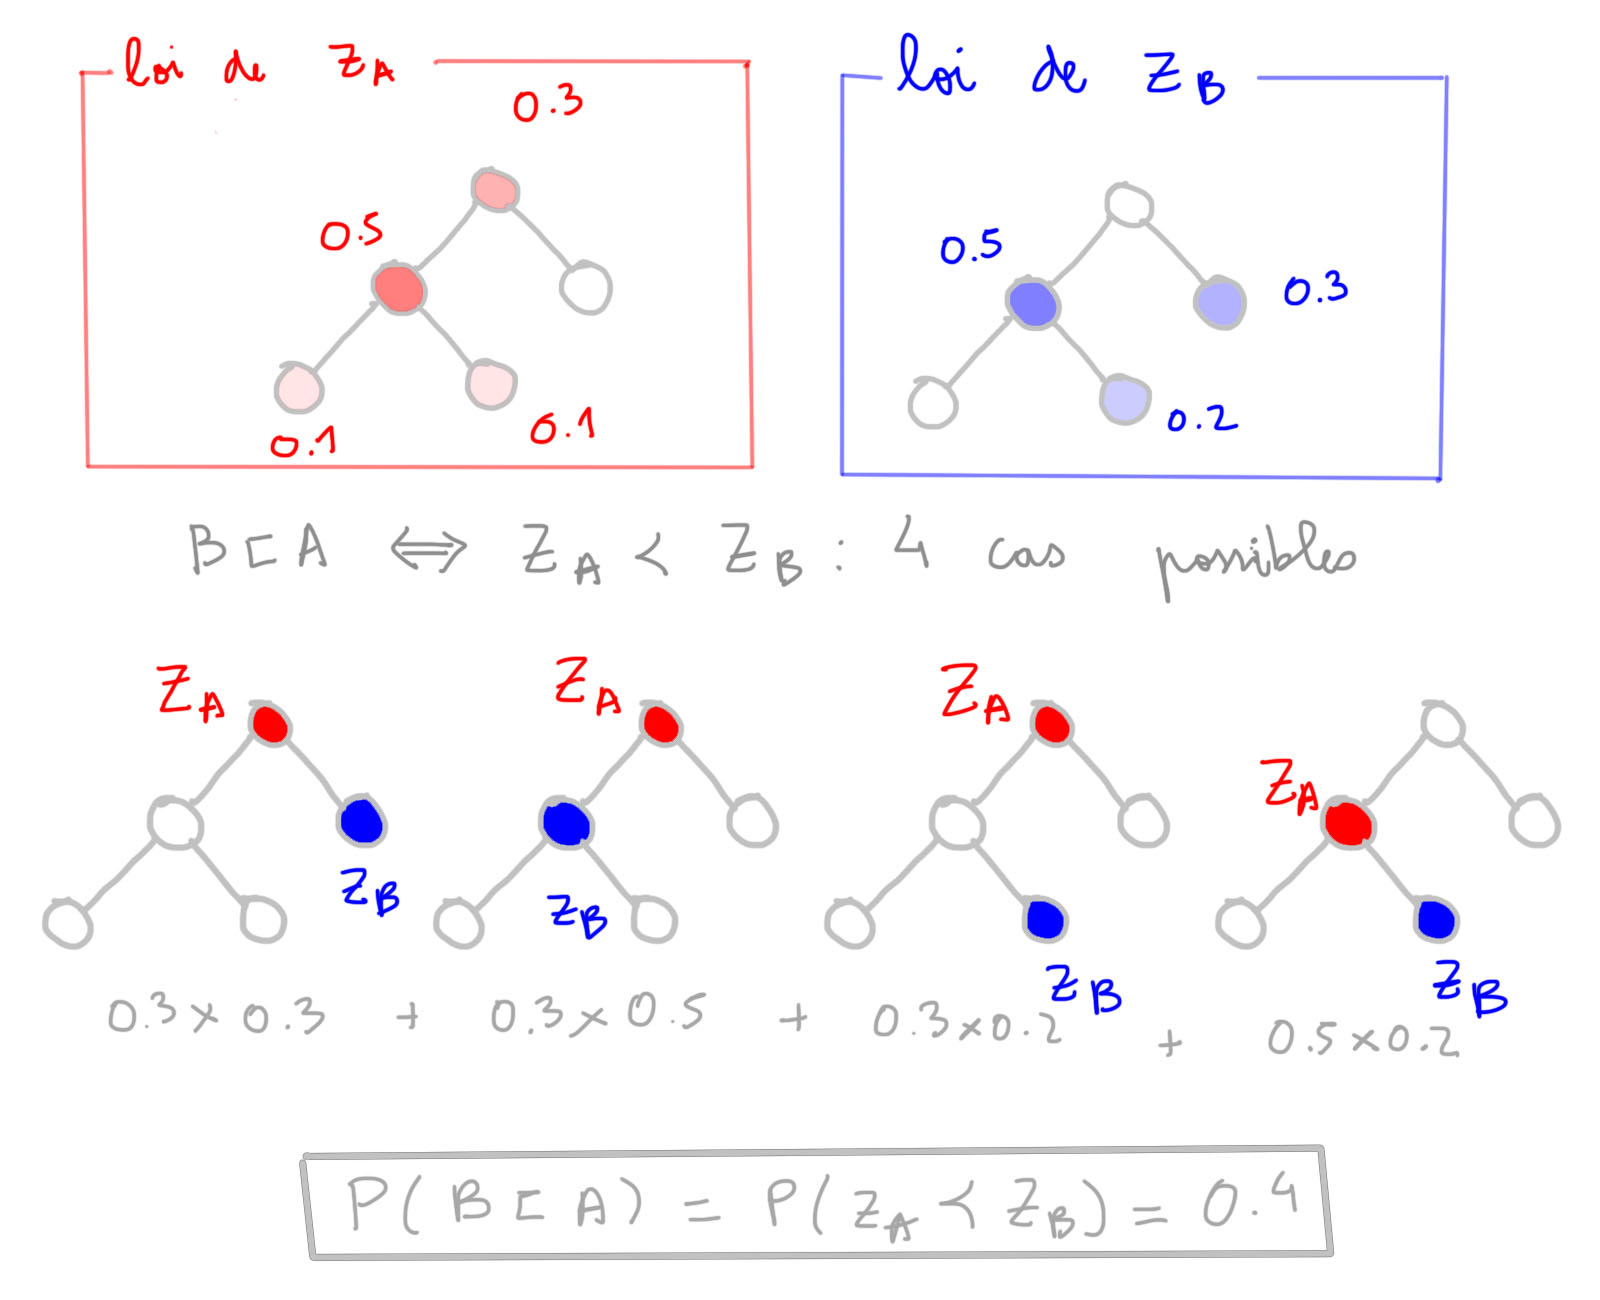
\includegraphics[width=0.7\textwidth]{img/softmapping.jpg}
    \caption[Principe de la méthode Soft Mapping]{Exemple de calcul de la probabilité de l'axiome $(B \sqsubset A)$ à partir de la loi de $Z_A$ (\textit{en haut à gauche}) et de la loi de $Z_B$ (\textit{en haut à droite}).}
    \label{fig:te-softmapping-example}
\end{figure}

Un exemple de calcul est illustré à la figure \ref{fig:te-softmapping-example}, dans le cas de deux classes $A$ et $B$ et d'un arbre de clustering de taille 4 et de profondeur 2.

% Ce compromis entre faux négatifs et faux positifs dépend 
% On pourra alors, dans l'étape de reconstruction de taxonomie, éliminer les axiomes trop incertains si l'on souhaite minimiser le nombre de faux positifs, ou au contraire garder des axiomes incertains si l'on veut minimiser le nombre de faux négatifs.
\paragraph{Formulation récursive}

Pour calculer ces probabilités pour chaque $t, t'$ sans sommer sur toutes les paires de clusters, on peut concevoir un algorithme récursif de type «diviser pour régner». Pour cela, il nous faut exprimer $P(t' \sqsubset t)$ sous forme récursive. On introduit donc une nouvelle quantité,  $P_C(t' \sqsubset t)$ : c'est, comme dans l'équation~\ref{eq:softmapping_2}, la probabilité de l'événement $t' \sqsubset t$ (c'est-à-dire de l'événément $Z_{t'} \subset Z_{t}$), mais restreint au cas où $Z_t$ et $Z_{t'}$ appartienent au sous-arbre $X[C]$.
\begin{equation}
    P_C(t' \sqsubset t) = P(Z_{t'} \subset Z_{t} \land Z_t, Z_{t'} \in X[C])
\end{equation}

Or appartenir au sous-arbre $X[C]$ est équivalent à être un successeur de $C$, on peut donc réécrire l'événement $(Z_{t'} \subset Z_{t}) \land (Z_t, Z_{t'} \in X[C])$ sous la forme $Z_{t'} \subset Z_{t} \subseteq C$. D'où :
\begin{align}
    P_C(t' \sqsubset t) &= P(Z_{t'} \subset Z_{t} \subseteq C) \nonumber \\
    &= \sum_{\substack{C, C' \in \succs(C) \\  C' \subset C}} P(Z_t = C)\cdot P(Z_{t'} = C) \label{eq:proba_subsumption}
\end{align}


% To compute these probabilities for all $t, t'$ without summing over all pairs of % clusters, we devise a divide-and-conquer algorithm. For this, we need a recursive % formulation of $P(t' \sqsubset t)$, so we introduce $P_C(t' \sqsubset t)$, the % probability of axiom $(t' \sqsubset t)$ computed on the subtree $X[C]$, for any given % cluster $C$. Similarly to equation~\ref{eq:softmapping_2}, it represents the % probability that the cluster $m(t)$ representing $t$ is a predecessor of  the cluster % $m(t')$ representing $t'$, with the additional condition that both $m(t)$ and $m(t')$ % must belong to the subtree $X[C]$ (that is, be successors of $C$):
% \begin{align}
%     P_C(t' \sqsubset t) &= P(C \preceq m(t) \prec m(t') % \text{ and } m(t),m(t') % \succeq C %, C \preceq m(t')
%     ) \nonumber \\
%     &= \sum_{\substack{C_A, C_B \in \succs(C) \\ C_A \prec C_B}} P(m(t) = C_A)\cdot % P(m(t') = C_B) 
%     \label{eq:proba_subsumption}
% \end{align}

Comme le sous-arbre $X[\texttt{racine}]$ est égal à l'arbre complet, on a $P_\texttt{racine}(t' \sqsubset t) = P(t' \sqsubset t)$, et $P(t' \sqsubset t)$ est la quantité que l'on cherche à calculer. De plus, si $C$ est une feuille, alors le sous-arbre $X[C]$ contient un unique élément, il est donc impossible d'avoir $Z_{t'} \subset Z_{t} \subseteq C$, et donc $P_C(t' \sqsubset t) = 0$ quels que soit $t$ et $t'$. 
Ainsi, on connait la valeur de $P_C$ sur les feuilles de l'arbre, et on souhaite calculer $P_\texttt{racine}$ : il suffit pour cela d'exprimer $P_C$ en fonction de $P_{\gauche(C)}$ et $P_{\droite(C)}$. On pourra alors calculer $P_\texttt{racine}(t \sqsubset t')$ récursivement, et on aura donc les probabilités $P(t \sqsubset t')$ recherchées.
% \ldots 
% \todo{Finir la réécriture de la section Soft Mapping dans le vocabulaire des v.a.}

Soit $L = \gauche(C)$ et $R = \droite(C)$ les sous-clusters gauche et droit de $C$. On peut remarquer qu'un successeur de $C$ est soit un successeur de $L$, soit un successeur de $R$, soit $C$ lui-même. Autrement dit, en notant $\sqcup$ l'union disjointe :
\begin{equation}
    \succs(C) = \succs(L) \sqcup \succs(R) \sqcup \{ C\}
\end{equation}
En suivant cette observation, on peut donc partager la somme~\ref{eq:proba_subsumption} en trois :
\begin{align}
P_{C}(t' \sqsubset t) = 
&
\sum_{\substack{C_A, C_B \in \succs(L) \\  C_B \subset C_A}} P(Z_t = C_A)\cdot P(Z_{t'} = C_B) 
\nonumber \\ 
&+ 
\sum_{\substack{C_A, C_B \in \succs(R) \\  C_B \subset C_A}} P(Z_t = C_A)\cdot P(Z_{t'} = C_B) 
\nonumber \\
&+ \displaystyle \sum_{C' \colon C' \subset C} P(Z_t = C) \cdot P(Z_{t'} = C_B) \nonumber \\
= {} & P_{L}(t' \sqsubset t) + P_{R}(t' \sqsubset t)  + P(Z_t=C)\cdot\sum_{\substack{C' \colon \\ C' \subset C}} P(Z_{t'} = C_B)
\label{eq:proba_over_subtree}
\end{align}

Cette équation fait apparaître le lien recherché entre $P_C$ d'un côté, et $P_L$ et $P_R$ de l'autre. On peut l'écrire de façon plus concise sous forme matricielle. Pour cela, définissons $n_T = | \mathcal{T} |$ le nombre de types distincts, $\mathbf{Q_C}$ une matrice de dimension $n_T \times n_T$ telle que sa coordonnée $(i, j)$ contienne $P_C(t_j \sqsubset t_i)$, et $\mathbf{p_C} = \left(P(Z_{t_i} = C)\right)_{i = 1, \ldots, n_T}$ le vecteur de probabilités du cluster $C$, de dimension $n_T$. 

Avec ces notations, notre objectif est de calculer $\bf{Q_\texttt{racine}}$, et donc d'obtenir une formule récursive reliant $\bf{Q_C}$ à $\bf{Q_L}$ et $\bf{Q_R}$. L'équation \ref{eq:proba_over_subtree} se réécrit matriciellement :
\begin{align}
    \mathbf{Q_C} &= \mathbf{Q_L} + \mathbf{Q_R} + \mathbf{p_C} \cdot \left(\sum_{C' \colon C' \subset C} \mathbf{p_{C'}} \right)^\top 
    \label{eq:recursive_q_formula}
\end{align}

À ce stade, l'équation \ref{eq:recursive_q_formula} est proche de la formulation récursive cherchée, mais il reste encore à éliminer la somme $\sum_{C' \colon C' \subset C} \mathbf{p_{C'}}$, parce qu'elle dépend de tous les successeurs stricts de $C$, et pas seulement de $C, L$ ou $R$. On note donc $\bf{s_C}$ cette somme :
\begin{align}
    \bf{s_C} &= \sum_{C' \colon C' \subset C} \mathbf{p_{C'}} \nonumber \\
            &= \sum_{C' \in \succs(C)^*} \mathbf{p_{C'}}
\end{align}
Cette somme est un vecteur de dimension $n_T$; sa $i$-ème coordonnée représente la probabilité pour le type $t_i$ d'être associé à un successeur strict de $C$, c'est-à-dire $P(Z_{t_i} \subset C)$. Or un successeur strict de $C$ est soit $L$ ou $R$, soit un successeur strict de $L$ ou $R$, ce qui s'exprime mathématiquement par :
\begin{equation}
    \succs(C)^* = \{L\} \sqcup \{R\} \sqcup \succs(L)^* \sqcup \succs(R)^*
\end{equation}

On peut donc réécrire $\bf{s_C}$ comme :
\begin{align}
    \mathbf{s_C} &= \mathbf{p_L} + \mathbf{p_R} + (\mathbf{s_L} + \mathbf{s_R}) \nonumber  \\
     &= (\mathbf{p_L}  + \mathbf{s_L}) + (\mathbf{p_R} + \mathbf{s_R})
    \label{eq:l_def}
\end{align}
Finalement, on définit la probabilité pour chaque type d'être associé à un successeur non-strict de $C$ : 
\begin{equation}
    \mathbf{u_C} = \mathbf{p_C} + \mathbf{s_C}
    \label{eq:def_uc}
\end{equation}
Cela permet de reformuler ainsi l'équation \ref{eq:l_def}:
\begin{equation}
    \mathbf{s_C} = \mathbf{u_L} + \mathbf{u_R}
    \label{eq:l_update}
\end{equation}

On a désormais nos équations de récurrences : \ref{eq:recursive_q_formula} pour $\bf{Q_C}$, \ref{eq:def_uc} pour $\bf{u_C}$ et \ref{eq:l_update} pour $\bf{s_C}$. Il reste à calculer les cas de base, c'est-à-dire les valeurs de $\bf{Q, u, s}$ pour les clusters feuilles. Si $C$ est une feuille, la probabilité pour un type $t$ d'être associé à un de ses successeurs stricts est nulle, puisque $C$ n'a aucun successeur strict. Pour la même raison, la probabilité pour qu'un axiome de subsumption $t' \sqsubset t$ soit vérifié dans le sous-arbre $X[C]$ est également zéro. Ainsi $\mathbf{s_C}$ et $\mathbf{Q_C}$ sont tous les deux nuls pour chaque cluster feuille. Quant à $\bf{u_C}$, sa valeur sur les feuilles peut être calculée par l'équation \ref{eq:def_uc}.

On peut finalement écrire les équations de récurrence pour $\mathbf{s_C}, \mathbf{Q_C}, \mathbf{u_C}$:
\begin{align}
    \mathbf{Q_C} &=
    \begin{cases}
      \mathbf{0}_{n_T,n_T} & \text{si $C$ est une feuille}\\
      \mathbf{p_C} \cdot \mathbf{s_C}^\top + \mathbf{Q_\text{gauche$(C)$}} + \mathbf{Q_\text{droite$(C)$}} & \text{sinon}
    \end{cases}  \\
  \mathbf{s_C} &=
    \begin{cases}
      \mathbf{o}_{n_T} & \text{si $C$ est une feuille}\\
      \mathbf{u_\text{gauche$(C)$}} + \mathbf{u_\text{droite$(C)$}} & \text{sinon}
    \end{cases}  \\
    \mathbf{u_C} &= \mathbf{p_C} + \mathbf{s_C}
\end{align}

Pour implémenter cet algorithme efficacement, on utilise la programmation linéaire. On note $D_C = (\mathbf{s_C}, \mathbf{Q_C}, \mathbf{u_C})$ l'ensemble des quantités calculées récursivement. Les clusters sont parcourus dans l'ordre inverse d'un parcours en profondeur, ce qui garantit que, lorsqu'on visite un cluster $C$, tous ses successeurs ont déjà été visités. Pour chaque cluster $C$, soit $C$ est une feuille, auquel cas on calcule $D_C$ à l'aide des formules d'initialisation précédentes; soit $C$ n'est pas une feuille, auquel cas ses deux sous-clusters $\gauche(C)$ et $\droite(C)$ ont déjà été visités et les quantités $D_{\gauche(C)}$ et $D_{\droite(C)}$ sont stockées dans le cache. Dans ce cas, on retire $D_{\gauche(C)}$ et $D_{\droite(C)}$ du cache (chaque cluster est visité une seule fois dans les équations de récurrence, donc plus aucun calcul ne dépend d'eux), on les utilise pour calculer $D_C$ selon les équations de récurrence précédentes, et on ajoute $D_C$ au cache. Le dernier cluster visité est \texttt{racine} : lorsque l'algorithme termine, le cache contient uniquement $D_\texttt{racine} = (\mathbf{s_\texttt{racine}}, \mathbf{Q_\texttt{racine}}, \mathbf{u_\texttt{racine}})$. On peut alors retourner la matrice de probabilité finale $\mathbf{Q_\texttt{racine}}$. Sa coordonnée $(i, j)$ contient la probabilité de l'axiome $(t_j \sqsubset t_i)$.
Pour un arbre binaire équilibré, cet algorithme garantit un cache de taille maximale $O(|\mathcal{T}|^2 \log_2(| \mathcal{C} |))$, avec $|\mathcal{T}| \ll | \mathcal{C} |$.


\subsection{Construction de la taxonomie}
\label{subsec:te-taxconstruction}

Une fois les types associés aux clusters, la taxonomie est construite en transformant la hiérarchie sur les clusters en une hiérarchie sur les types. Dans le cas de la méthode \textit{Hard Mapping}, l'injectivité de l'association permet de réaliser facilement cette transformation. La taxonomie prédite $\Tpred$ contient tous les types $t \in \cal{T}$, et elle contient l'axiome $t' \sqsubset t$ si et seulement si les clusters $m(t')$ et $m(t)$ associés à $t$ et $t'$ sont succcesseurs l'un de l'autre ($m(t') \subset m(t)$), sans qu'il existe un cluster étiquetté entre $m(t)$ et $m(t')$ :
\begin{equation}
    \Tpred = (\cal{T}, \{t' \sqsubset t : m(t') \subset m(t) \text{ et } \forall C \in \cal{C},  m(t') \subseteq C \subseteq m(t) \implies C \notin m(\cal{T}) \})
    \label{eq:te-extract-tax-from-mapping}
\end{equation}

\begin{figure}[h]
    \centering
    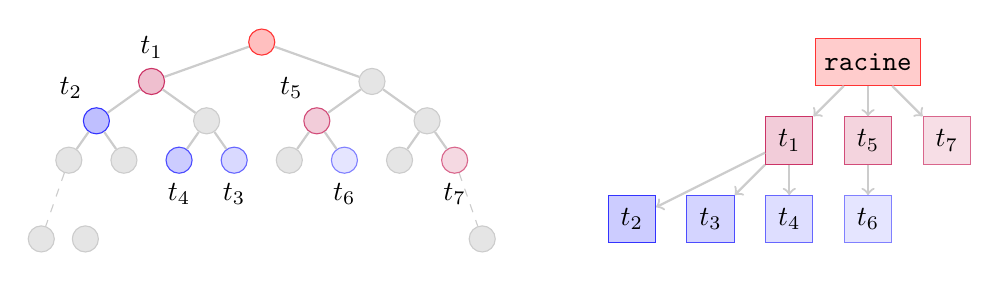
\begin{tikzpicture}
    [   
    cnode/.style={draw=gray!40,fill=gray!20,minimum width=0.2mm,circle},
    colnode/.style={draw=red!80,fill=red!40,minimum width=0.2mm,circle},
    cline/.style={gray!40,thick},
    rnode/.style={draw=gray!40,fill=gray!20,minimum width=6mm, minimum height=6mm, rectangle},
    recnode/.style={fill=#1,minimum width=0.2mm,circle},
    r1node/.style={draw=#1!80,fill=#1!25,minimum width=0.2mm,circle},
    r2node/.style={draw=#1!70,fill=#1!20,minimum width=0.2mm,circle},
    r3node/.style={draw=#1!60,fill=#1!15,minimum width=0.2mm,circle},
    r4node/.style={draw=#1!50,fill=#1!10,minimum width=0.2mm,circle},
    t1node/.style={draw=#1!80,fill=#1!20,minimum width=6mm, minimum height=6mm, rectangle},
    t2node/.style={draw=#1!70,fill=#1!17,minimum width=6mm, minimum height=6mm, rectangle},
    t3node/.style={draw=#1!60,fill=#1!13,minimum width=6mm, minimum height=6mm, rectangle},
    t4node/.style={draw=#1!50,fill=#1!10,minimum width=6mm, minimum height=6mm, rectangle},
    ]
    
    %
    % CLUSTERING TREE
    %
    
    \def\stepx{0.7};
    \def\stepy{0.5};
    
    \node[r3node=blue, label=270:$t_3$] (000) at (-0.5*\stepx,-2*\stepy) {};
    \node[r2node=blue, label=270:$t_4$] (001) at (-1.5*\stepx,-2*\stepy) {};
    \node[cnode] (010) at (-2.5*\stepx,-2*\stepy) {};
    \node[cnode] (011) at (-3.5*\stepx,-2*\stepy) {};
    \node[cnode] (100) at (0.5*\stepx,-2*\stepy) {};
    \node[r4node=blue, label=270:$t_6$] (101) at (1.5*\stepx,-2*\stepy) {};
    \node[cnode] (110) at (2.5*\stepx,-2*\stepy) {};
    \node[r3node=purple, label=270:$t_7$] (111) at (3.5*\stepx,-2*\stepy) {};
    
    \node[r1node=blue, label=110:$t_2$] (00) at (-3*\stepx,-\stepy) {};
    \node[cnode] (01) at (-1*\stepx,-\stepy) {};
    \node[r2node=purple, label=110:$t_5$] (10) at (1*\stepx,-\stepy) {};
    \node[cnode] (11) at (3*\stepx,-\stepy) {};
    
    \node[r1node=purple, label=90:$t_1$] (0) at (-2*\stepx,0*\stepy) {};
    \node[cnode] (1) at (2*\stepx,0*\stepy) {};
    
    \node[r1node=red] (root) at (0,\stepy) {};
    
    
    \def\minx{-5.5*\stepx};
    
    \node[cnode] (t1) at (-4*\stepx,-4*\stepy) {};
    \node[cnode] (t2) at (-3.2*\stepx,-4*\stepy) {};
    \node[cnode] (tn) at (4*\stepx,-4*\stepy) {};
    
    \draw[cline] (root) -- (0) {};
    \draw[cline] (root) -- (1) {};
    
    \draw[cline] (00) -- (0) {};
    \draw[cline] (10) -- (1) {};
    \draw[cline] (01) -- (0) {};
    \draw[cline] (11) -- (1) {};
    
    \draw[cline] (01) -- (000) {};
    \draw[cline] (01) -- (001) {};
    \draw[cline] (00) -- (010) {};
    \draw[cline] (00) -- (011) {};
    \draw[cline] (10) -- (100) {};
    \draw[cline] (10) -- (101) {};
    \draw[cline] (11) -- (110) {};
    \draw[cline] (11) -- (111) {};
    
    \draw[dashed,gray!40] (011) -- (t1) {};
    \draw[dashed,gray!40] (111) -- (tn) {};
    
    %
    % EXTRACTED TAXONOMY
    %
    
    \def\offsety{0.5*\stepy}; %-6*\stepy};
    \def\offsetx{11*\stepx};

    \node[t1node=red] (l11) at (0+\offsetx, \offsety) {\texttt{racine}};
    
    \node[t1node=purple] (l21) at (-1+\offsetx, \offsety-1) {$t_1$};
    \node[t2node=purple] (l22) at (0+\offsetx, \offsety-1) {$t_5$};
    \node[t3node=purple] (l23) at (1+\offsetx, \offsety-1) {$t_7$};
    
    \node[t1node=blue] (l31) at (-3 + \offsetx, \offsety-2) {$t_2$};
    \node[t2node=blue] (l32) at (-2 + \offsetx, \offsety-2) {$t_3$};
    \node[t3node=blue] (l33) at (-1 + \offsetx, \offsety-2) {$t_4$};
    \node[t4node=blue] (l34) at  (0 + \offsetx, \offsety-2) {$t_6$};
    
    \draw[->, gray!40, thick] (l11) -- (l21) {};
    \draw[->, gray!40, thick] (l11) -- (l22) {};
    \draw[->, gray!40, thick] (l11) -- (l23) {};
    \draw[->, gray!40, thick] (l21) -- (l31) {};
    \draw[->, gray!40, thick] (l21) -- (l32) {};
    \draw[->, gray!40, thick] (l21) -- (l33) {};
    \draw[->, gray!40, thick] (l22) -- (l34) {};
\end{tikzpicture}
    \caption[Extraction de taxonomie selon la méthode Hard Mapping]{Extraction de taxonomie à partir d'un arbre de clustering étiquetté (méthode Hard Mapping).}
    \label{fig:te-hm-extraction}
\end{figure}


Pour rappel, $m(\cal{T})$ désigne l'image de $\cal{T}$ par $m$, c'est-à-dire l'ensemble des clusters qui sont associés à un type :
\begin{equation}
    m(\cal{T}) = \{ C \in \cal{C}, \exists t \in \cal{T}, m(t) = C \}
\end{equation}
Autrement dit, pour chaque type $t'$, on récupère le cluster associé $m(t')$, et on remonte vers la racine en cherchant le premier prédécesseur de $m(t')$ qui soit associé à un type. Si un tel prédécesseur $m(t)$ existe, on ajoute à $\Tpred$ l'axiome de subsumption $t' \sqsubset t$. Ce processus est décrit à la figure \ref{fig:te-hm-extraction}.



Dans le cas du \textit{Soft Mapping}, on récupère une liste d'axiomes de subsumption $t' \sqsubset t$ qui ne constituent pas nécessairement une taxonomie, et ce pour deux raison. D'une part, la condition d'injectivité qui existe pour la méthode de \textit{Hard Mapping} n'existe pas ici, si bien que l'on peut extraire à la fois les axiomes $t \sqsubset t'$ et $t' \sqsubset t$. D'autre part, même dans le cas idéal – et théorique – où l'algorithme d'association donnerait une probabilité $1$ aux axiomes effectivement valides et $0$ aux axiomes invalides, le résultat ne serait pas un arbre mais la clôture transitive d'un arbre. En effet, par construction de l'algorithme, on n'extrait pas uniquement l'axiome $t \sqsubset t'$ pour l'immédiat parent de $t$, mais tous les axiomes $t \sqsubset t_i$ pour les axiomes $t_i$ tels que $t \sqsubset t_1 \sqsubset t_2 \ldots \sqsubset t_k$. Cela revient à supprimer la clause $\forall C \in \cal{C},  m(t') \subseteq C \subseteq m(t) \implies C \notin m(\cal{T})$ de l'équation \ref{eq:te-extract-tax-from-mapping}. Pour ces deux raisons, il est nécessaire d'opérer un filtrage avant de pouvoir obtenir une taxonomie valide : d'une part en éliminant les axiomes susceptibles de créer des cycles dans la taxonomie, d'autre part en calculant la réduction transitive (l'opération inverse de la clôture transitive).

\begin{figure}
    \centering
    % 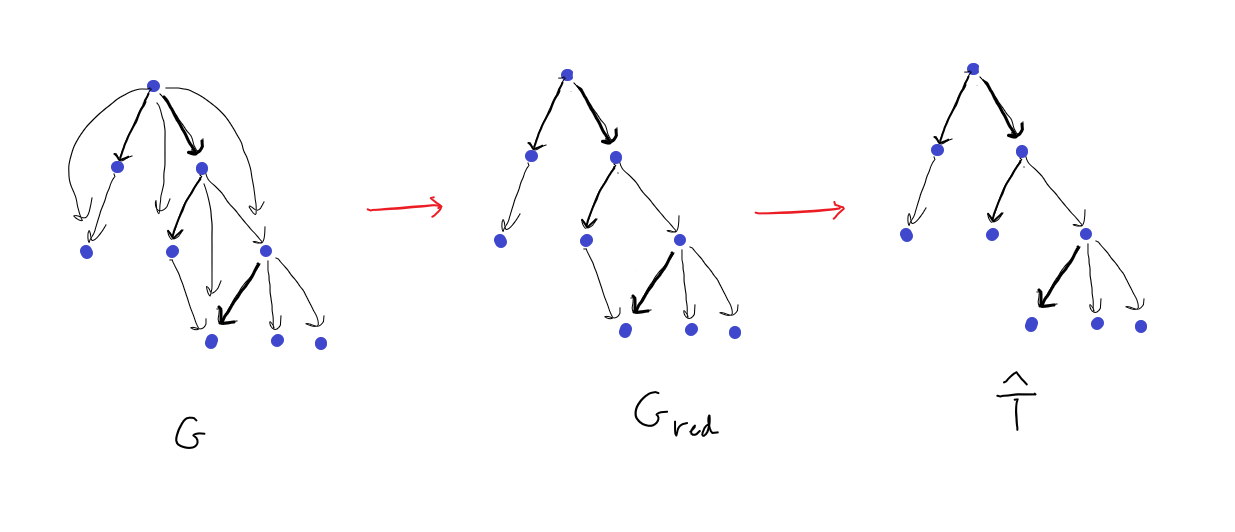
\includegraphics[width=\textwidth]{img/softmapping_extraction.png}
    \begin{tikzpicture}[
  box/.style={draw=gray, thick, align=center},
  arrow/.style={->, shorten >=3pt},
  node/.style={draw=gray, fill=gray!20},
  hnode/.style={draw=accent1, fill=accent1!20},
  snode/.style={draw=accent1, fill=accent1!20, very thick},
  point/.style={circle, draw=accent2, fill=accent2, node distance=1.3cm and 0.5cm, inner sep=0, minimum height=0.25cm},
  verysure/.style={very thick},
  sure/.style={thick},
  unsure/.style={line width=0.01cm, draw=black!50},
  medsure/.style={draw=black!80}
]

\def\y{1.5cm};
\def\x{0.5cm};

\begin{scope}

\node[point] (root) at (0, 0) {};
\node[point, below left=of root] (a1) {};
\node[point, below right=of root] (a2) {};
\node[point, below left=of a1] (b1) {};
\node[point, below left=of a2] (b2) {};
\node[point, below right=of a2] (b3) {};
\node[point, below left=of b3] (c1) {};
\node[point, below=of b3] (c2) {};
\node[point, below right=of b3] (c3) {};

\draw[arrow, verysure] (root) to (a1);
\draw[arrow, sure] (root) to (a2);
\draw[arrow, unsure] (root) to (b2);
\draw[arrow, medsure] (root) to[bend left] (b3);
\draw[arrow, unsure] (root) to[bend right] (b1);
\draw[arrow] (a1) to (b1);
\draw[arrow] (a2) to (b2);
\draw[arrow, sure] (a2) to (b3);
\draw[arrow, medsure] (a2) to (c1);
\draw[arrow, unsure] (b2) to (c1);
\draw[arrow, verysure] (b3) to (c1);
\draw[arrow, medsure] (b3) to (c2);
\draw[arrow] (b3) to (c3);

\node[right=of a2] (l1) {};
\node[right=2cm of l1] (l2) {};
\draw[very thick, red, ->] (l1) to (l2);

\node[below=2.6cm of b2, anchor=south] {$G$};
\end{scope}

\begin{scope}[xshift=6cm]

\node[point] (root) at (0, 0) {};
\node[point, below left=of root] (a1) {};
\node[point, below right=of root] (a2) {};
\node[point, below left=of a1] (b1) {};
\node[point, below left=of a2] (b2) {};
\node[point, below right=of a2] (b3) {};
\node[point, below left=of b3] (c1) {};
\node[point, below=of b3] (c2) {};
\node[point, below right=of b3] (c3) {};

\draw[arrow, verysure] (root) to (a1);
\draw[arrow, sure] (root) to (a2);
% \draw[arrow, unsure] (root) to (b2);
% \draw[arrow, medsure] (root) to[bend left] (b3);
% \draw[arrow, unsure] (root) to[bend right] (b1);
\draw[arrow] (a1) to (b1);
\draw[arrow] (a2) to (b2);
\draw[arrow, sure] (a2) to (b3);
% \draw[arrow, medsure] (a2) to (c1);
\draw[arrow, unsure] (b2) to (c1);
\draw[arrow, verysure] (b3) to (c1);
\draw[arrow, medsure] (b3) to (c2);
\draw[arrow] (b3) to (c3);

\node[right=of a2] (l1) {};
\node[right=2cm of l1] (l2) {};
\draw[very thick, red, ->] (l1) to (l2);

\node[below=2.6cm of b2, anchor=south] {$G_\textrm{red}$};
\end{scope}

\begin{scope}[xshift=12cm]

\node[point] (root) at (0, 0) {};
\node[point, below left=of root] (a1) {};
\node[point, below right=of root] (a2) {};
\node[point, below left=of a1] (b1) {};
\node[point, below left=of a2] (b2) {};
\node[point, below right=of a2] (b3) {};
\node[point, below left=of b3] (c1) {};
\node[point, below=of b3] (c2) {};
\node[point, below right=of b3] (c3) {};

\draw[arrow, verysure] (root) to (a1);
\draw[arrow, sure] (root) to (a2);
% \draw[arrow, unsure] (root) to (b2);
% \draw[arrow, medsure] (root) to[bend left] (b3);
% \draw[arrow, unsure] (root) to[bend right] (b1);
\draw[arrow] (a1) to (b1);
\draw[arrow] (a2) to (b2);
\draw[arrow, sure] (a2) to (b3);
% \draw[arrow, medsure] (a2) to (c1);
%\draw[arrow, unsure] (b2) to (c1);
\draw[arrow, verysure] (b3) to (c1);
\draw[arrow, medsure] (b3) to (c2);
\draw[arrow] (b3) to (c3);

\node[below=2.6cm of b2, anchor=south] {$\hat{T}$};
\end{scope}

\end{tikzpicture}
    \caption[Extraction de taxonomie à partir d'un graphe acyclique]{Extraction de taxonomie à partir d'une liste pondérée d'axiomes (méthode Soft Mapping) : un graphe acyclique est construit avec les axiomes les plus probables (gauche), sa réduction transitive est calculée (milieu), puis le graphe est transformé en arbre en retirant les arêtes de probabilités minimales (droite). L'épaisseur des arêtes représente la probabilité.}
    \label{fig:softmapping-extraction}
\end{figure}

Pour cela, on construit un graphe $G$ des axiomes à conserver. Chaque axiome extrait est examiné, par ordre de probabilité décroissante. Pour chaque axiome $\alpha$, si ajouter $\alpha$ à $G$ crée un cycle, on rejete $\alpha$. Sinon, on l'ajoute effectivement à $G$. Par construction, le graphe $G$ ainsi obtenu est un graphe orienté acyclique (ou DAG en anglais, pour \textit{direct acyclic graph}) : il est bien acyclique car le graphe de départ est vide donc acyclique, et car il reste acyclique à chaque étape; il est orienté car l'axiome de subsumption $t \sqsubset t'$ est différent de l'axiome inverse $t' \sqsubset t$, il y a donc bien une orientation des arêtes de $G$. 

Ensuite, on calcule la réduction transitive $G_{red}$ du graphe $G$ : c'est le plus petit graphe $G_{red}$ tel qu'il existe un chemin de $t$ vers $t'$ dans $G_{red}$ si et seulement si il existe un chemin de $t$ vers $t'$ dans $G$. Enfin, pour tout type $t$ qui a un degré entrant supérieur à 1, c'est-à-dire qui est impliqué dans au moins deux axiomes $t \sqsubset t'$ et $t\sqsubset t''$, on supprime tous les axiomes de la forme $t \sqsubset t'$ à l'exception de celui de probabilité maximale. Le résultat est la taxonomie extraite $\Tpred$. Le processus est représenté à la figure \ref{fig:softmapping-extraction}.


\section{Évaluation et discussion}
\label{sec:te-evaluation}

\subsection{Données}
\label{sec:te-data}

Comme dans le chapitre précédent, on utilise le graphe DBpédia, dans sa version de 2016-10. En plus du graphe de connaissances proprement dit, DBpédia dispose d'une ontologie\footnote{qui peut être consultée à l'adresse \href{http://mappings.dbpedia.org/server/ontology/classes/}{mappings.dbpedia.org/server/ontology/classes/} dans une version légèrement mise à jour, ou téléchargée au format OWL à l'adresse \href{http://downloads.dbpedia.org/2016-10/dbpedia\_2016-10.owl}{downloads.dbpedia.org/2016-10/dbpedia\_2016-10.owl}}, qui contient 455 classes ayant au moins une instance. Toutes les classes héritent d'une classe racine \texttt{owl:Thing} (classe de niveau 0); la profondeur maximale d'une classe est 6. Pour évaluer notre approche, on n'utilise pas toute l'ontologie DBpédia, mais une version simplifiée restreinte aux classes fréquentes. %(à discuter)
%On extrait donc un sous-arbre de la taxonomie DBpédia complète, constituée de classes suffisamment fréquentes.
Pour extraire cette sous-taxonomie, on fixe la profondeur maximale à $p_{\max}=3$, le nombre maximal de sous-classes par classe à $n_c=7$ et le nombre minimal d'éléments par classe à $n_e=500$. En partant de la classe racine \texttt{owl:Thing}, on ajoute récursivement les sous-classes $S$ d'une classe $C$, par ordre décroissant d'effectif (on commence par ajouter les sous-classes qui contiennent le plus d'éléments), à condition que : 
\begin{itemize}
    \item $S$ contienne au moins $n_e$ entités
    \item la profondeur de $S$ soit au plus $p_{\max}$
    \item $C$ ait moins de $n_c$ sous-classes
\end{itemize}

Cette taxonomie sera nommée par la suite \textsc{DBpédia-Fréq}. Elle contient sept classes de niveau 1, qui sont \texttt{Agent}, \texttt{Event}, \texttt{MeanOfTransportation}, \texttt{Place}, \texttt{Species}, \texttt{SportsSeason}, \texttt{Work}; 25 classes de niveau 2, et 52 classes de niveau 3. Cette taxonomie, quoique simplifiée, couvre 75\% des triplets \texttt{rdf:type} de DBpédia. Les valeurs des paramètres $p_{\max}, n_c, n_e$ ont été choisis empiriquement de sorte à atteindre ce seuil de couverture. 

Une fois que l'on dispose de cette taxonomie de référence \textsc{DBpédia-Fréq}, on prélève aléatoirement dans le graphe des instances de chacune des classes de la taxonomie; on obtient un jeu de données $\cal{D}$ comportant $N = 51 418$ instances, chacune étant ensuite représentée par un plongement vectoriel de dimension $d=50$. L'objectif est alors de reconstituer \textsc{DBpédia-Fréq} à partir de $\cal{D}$.


%L'ontologie DBpédia comporte un ensemble de classes et de sous-classes qui forment un arbre dont on peu trouver le détail à l'adresse \href{http://mappings.dbpedia.org/server/ontology/classes/}{http://mappings.dbpedia.org/server/ontology/classes/}. Comme on peut le voir, toutes les classes héritent d'une seule classe racine \texttt{owl:Thing} (classe de niveau 0); la profondeur maximale d'une sous-classe est 6. On peut difficilement utiliser toute l'ontologie pour le clustering, car certaines classes très spécifiques contiennent trop peu d'éléments [par exemple, seulement 7 éléments sont de type \texttt{dbo:Star}). On cherche donc à extraire un sous-arbre qui soit (a) suffisamment profond pour modéliser une base de connaissance du monde réel et tel que (b) chaque classe contienne un nombre minimal d'éléments. 



% À partir de cette taxonomie, on tire pour chaque classe feuille un ensemble d'instances DBpédia qui y appartienne. On obtient alors $N=51 418$  instances. Chaque instance est représentée par son plongement, de dimension $d=50$. Le jeu de données consiste donc en une matrice réelle de dimension $51 418 \times 50$.

\subsection{Méthode d'évaluation}
\label{subsec:te-evaluation}

On évalue notre méthode en faisant varier le modèle de plongement employé, le type de regroupement hiérarchique et la méthode d'association type-cluster. Les modèles de plongement expérimentés sont TransE, TransD, TransH, ComplEx, DistMult et RDF2Vec. Le regroupement hiérarchique se fait avec un des quatre critères de liaison cités (saut minimum, moyen, maximum, critère de Ward) et l'une des trois distances suivantes : euclidienne, cosinus, $L_1$. % soit avec le critère de Ward basé sur la distance euclidienne, soit par liaison moyenne avec la distance cosinus – le choix de ces deux combinaisons de paramètres est discuté dans la section \ref{sec:te-hp}. 
La méthode d'association est soit \textit{Hard Mapping}, soit \textit{Soft Mapping}. On compare ces résultats avec ceux obtenus par la méthode TIEmb \cite{ristoski2017large} (présentée à la section \ref{subsec:litt-tiemb}, page \pageref{subsec:litt-tiemb}); pour cette méthode également, on expérimente avec les distances euclidienne, cosinus et $L_1$. 

Pour comparer une taxonomie prédite $\Tpred$ avec la taxonomie de référence de \textsc{DBpédia-Freq}, notée ici $T^*$, on mesure la différence entre les axiomes de subsumption prédits et les axiomes de référence en calculant la précision (nombre d'axiomes prédits qui sont vrais), le rappel (nombre de vrais axiomes qui sont correctement prédits), et la mesure $F_1$ (moyenne géométrique de la précision et du rappel). On calcule également la clôture transitive de $\Tpred$ et $T^*$ : la clôture transitive d'un arbre $T$ est le graphe $T^+$ qui contient les mêmes sommets que $T$ et dont les arêtes sont définies par $t \sqsubset t' \iff \exists t_1, \ldots t_k, (t \sqsubset t_1), (t_1 \sqsubset t_2), \ldots, (t_k \sqsubset t') \in T$. C'est donc le graphe obtenu en reliant un sommet $t$ à tous ses prédécesseurs dans $T$. Une fois ces clôtures transitives calculées, on évalue à nouveau la différence entre les axiomes de $\Tpred^+$ et ceux de $(T^*)^+$ en terme de précision, de rappel et de mesure $F_1$. Ces deux modes d'évaluation sont appelés respectivement \textit{évaluation directe} et \textit{évaluation transitive}.

Ces deux modes d'évaluation – directe et transitive – sont nécessaires pour évaluer correctement la proximité d'une taxonomie prédite avec une taxonomie de référence, car ils ne mesurent pas la même chose. Prenons le cas où le modèle d'extraction prédit correctement la plupart des axiomes mais commet des erreurs sur les axiomes de haut niveau (proches de la racine, par exemple en prédisant à tort l'axiome $\dbo{Person} \sqsubset \dbo{Event}$). Comme la majorité des axiomes sont corrects, la mesure $F_1$ directe est élevée; toutefois, après clôture transitive, l'erreur de haut niveau se propage dans tout le sous-arbre : dans notre exemple, toutes les sous-classe de \dbo{Person} seront incorrectement considérées comme des sous-classes de \dbo{Event}, ce qui fera chuter la précision et donc la mesure $F_1$. À l'inverse, considérons le cas où un modèle extrait correctement les axiomes de haut niveau mais ne parvient pas à reproduire les axiomes de plus bas niveau – par exemple en prédisant $\dbo{SoccerPlayer} \sqsubset \dbo{Person}$ et $\dbo{Athlete} \sqsubset \dbo{Person}$ au lieu de $\dbo{SoccerPlayer} \sqsubset \dbo{Athlete} \sqsubset \dbo{Person}$. Dans ce cas, la mesure $F_1$ transitive est élevée, car la majorité des axiomes transitifs de référence sont correctement prédits, mais la mesure $F_1$ directe est basse, car les axiomes directs manquent. % En un sens, la mesure directe donne une évaluation locale de la prédiction


\subsection{Résultats}
\label{subsec:te-results}

Les résultats principaux sont présentés dans le tableau \ref{tab:te-results} pour les modèles ComplEx, DistMult, RDF2Vec et TransE. On y présente les résultats pour les méthodes Hard Mapping et Soft Mapping avec, pour chacune, deux variantes de regroupement hiérarchique : l'une avec distance cosinus et critère du saut moyen, l'autre avec distance euclidienne et critère de Ward. Pour les modèles Soft Mapping, les paramètres sont fixés à $\beta = 100$ et $t=0.1$ (ces choix sont discutés dans la section \ref{subsec:te-hp-softmapping}). Pour la méthode TIEmb, on se restreint également aux distances cosinus et euclidienne. Les résultats pour les autres modèles de plongement, métriques et critères de liaison sont présentés en annexe.

% Si l'on considère le $F_1$ moyen comme 
Du point de vue du $F_1$ moyen, le meilleur modèle est \textit{Soft Mapping} (SM) avec TransE et distance cosinus; ce modèle obtient d'ailleurs le $F_1$ le plus élevé sur chacune des trois évaluations. Ce modèle est suivi, dans l'ordre décroissant, par \textit{Hard Mapping} (HM) avec TransE et distance cosinus, SM avec TransE et distance euclidienne, TIEmb et les distances cosinus puis euclidiennes, et HM avec TransE et distance euclidienne. Tous ces modèles obtiennent un $F_1$ moyen supérieur à $0,75$.

En moyenne, la méthode SM obtient des résultats supérieurs à HM et à TIEmb. TIEmb est inférieur aux méthodes SM et HM sur tous les modèles de plongement à l'exception de RDF2Vec, où il obtient de meilleurs scores. 

% Les modèles qui obtiennent un $F_1$ moyen supérieur à 0.75 sont, par ordre décroissant, SM et HM avec TransE et la distance cosinus, SM avec TransE et la distance euclidienne, TIEmb avec TransE et les distances cosinus puis euclidienne, et HM avec TransE et la distance euclidienne. 


Si l'on évalue les modèles de plongement sur leur capacité à intégrer géométriquement l'information taxonomique, la hiérachie entre modèles est nette : TransE obtient les meilleurs résultats, quelle que soit la méthode d'extraction ou la distance utilisée; RDF2Vec couplé à TIEmb obtient de bons résultats pour l'évaluation directe, ce qui indique une capacité à intégrer correctement les hiérarchies locales, mais commet des erreurs de haut niveau qui grèvent ses résultats moyens; ComplEx et DistMult sont nettement inférieurs à TransE, avec un léger avantage pour ComplEx.


% TODO à affiner

\begin{table}
    \centering
    \caption[Évaluation de trois méthodes d'extraction de taxonomie]{
    Évaluation de notre approche et de TIEmb sur \textsc{DBpedia-Freq}, pour différents modèles de plongement. $p, r, F_1$ désignent respectivement la précision, le rappel et la mesure $F_1$. \textit{cos} et \textit{euc} indiquent les distances cosinus et euclidienne. Les résultats de la section \textit{Moyenne} sont obtenus en calculant la moyenne des évaluations directe et transitive.}
    \begin{adjustwidth}{-1in}{-1in}
        \begin{center}
            \begin{tabular}{|lll|ccc|ccc|ccc|}
    \hline 
                               &      &          & \multicolumn{3}{c|}{Directe}              & \multicolumn{3}{c|}{Transitive}     & \multicolumn{3}{c|}{Moyenne}     \\
        Méthode	&	Plongements	&	Distance	&	$p$	&	$r$	&	$F$	&	$p$	&	$r$	&	$F1$	&	$p$	&	$r$	&	$F1$	\\	
\hline \multirow{8}{*}{TIEmb}	&	\multirow{2}{*}{ComplEx}	&	cos	&	0.38	&	0.38	&	0.38	&	0.28	&	0.57	&	0.37	&	0.33	&	0.48	&	0.38	\\
	&		&	euc	&	0.39	&	0.42	&	0.4	&	0.34	&	0.8	&	0.48	&	0.37	&	0.61	&	0.44	\\[2pt] 
	&	\multirow{2}{*}{DistMult}	&	cos	&	0.26	&	0.27	&	0.26	&	0.19	&	0.44	&	0.27	&	0.23	&	0.36	&	0.27	\\
	&		&	euc	&	0.37	&	0.41	&	0.39	&	0.33	&	0.79	&	0.47	&	0.35	&	0.60	&	0.43	\\[2pt] 
	&	\multirow{2}{*}{RDF2Vec}	&	cos	&	0.77	&	\textbf{0.84}	&	0.81	&	0.43	&	0.87	&	0.57	&	0.60	&	0.86	&	0.69	\\
	&		&	euc	&	0.70	&	0.77	&	0.73	&	0.30	&	0.73	&	0.42	&	0.50	&	0.75	&	0.58	\\[2pt] 
	&	\multirow{2}{*}{TransE}	&	cos	&	0.77	&	0.72	&	0.74	&	0.83	&	0.89	&	0.86	&	0.80	&	0.81	&	0.80	\\
	&		&	euc	&	0.76	&	0.75	&	0.76	&	0.7	&	0.9	&	0.79	&	0.73	&	0.83	&	0.78	\\[2pt] 
\hline \multirow{8}{*}{\shortstack[c]{Hard Mapping \\ (HM)}}	&	\multirow{2}{*}{ComplEx}	&	cos	&	0.53	&	0.5	&	0.52	&	0.78	&	0.7	&	0.74	&	0.66	&	0.60	&	0.63	\\
	&		&	euc	&	0.51	&	0.44	&	0.47	&	0.87	&	0.52	&	0.65	&	0.69	&	0.48	&	0.56	\\[2pt] 
	&	\multirow{2}{*}{DistMult}	&	cos	&	0.55	&	0.47	&	0.5	&	0.73	&	0.57	&	0.64	&	0.64	&	0.52	&	0.57	\\
	&		&	euc	&	0.43	&	0.36	&	0.39	&	0.75	&	0.54	&	0.63	&	0.59	&	0.45	&	0.51	\\[2pt] 
	&	\multirow{2}{*}{RDF2Vec}	&	cos	&	0.60	&	0.44	&	0.50	&	0.88	&	0.50	&	0.63	&	0.74	&	0.47	&	0.57	\\
	&		&	euc	&	0.60	&	0.53	&	0.56	&	0.89	&	0.64	&	0.74	&	0.74	&	0.58	&	0.65	\\[2pt] 
	&	\multirow{2}{*}{TransE}	&	cos	&	0.82	&	0.8	&	0.81	&	0.97	&	0.89	&	\textbf{0.93}	&	\textbf{0.90}	&	0.85	&	0.87	\\
	&		&	euc	&	0.73	&	0.67	&	0.7	&	\textbf{0.99}	&	0.68	&	0.8	&	0.86	&	0.68	&	0.75	\\[2pt] 
\hline \multirow{8}{*}{\shortstack[c]{Soft Mapping \\ (SM)}}	&	\multirow{2}{*}{ComplEx}	&	cos	&	0.52	&	0.48	&	0.5	&	0.89	&	0.7	&	0.79	&	0.71	&	0.59	&	0.65	\\
	&		&	euc	&	0.51	&	0.44	&	0.47	&	0.84	&	0.6	&	0.7	&	0.68	&	0.52	&	0.59	\\[2pt] 
	&	\multirow{2}{*}{DistMult}	&	cos	&	0.5	&	0.44	&	0.47	&	0.87	&	0.65	&	0.74	&	0.69	&	0.55	&	0.61	\\
	&		&	euc	&	0.48	&	0.42	&	0.45	&	0.86	&	0.65	&	0.74	&	0.67	&	0.54	&	0.60	\\[2pt] 
	&	\multirow{2}{*}{TransE}	&	cos	&	\textbf{0.83}	&	0.81	&	\textbf{0.82}	&	0.93	&	\textbf{0.93}	&	\textbf{0.93}	&	0.88	&	\textbf{0.87}	&	\textbf{0.88}	\\
	&		&	euc	&	0.78	&	0.77	&	0.77	&	0.98	&	0.87	&	0.92	&	0.88	&	0.82	&	0.85	\\[2pt] 
\hline
    \end{tabular}
            \label{tab:te-results} 
        \end{center}
    \end{adjustwidth}
\end{table}



\subsection{Discussion}
\label{subsec:te-discussion}


On peut trouver étonnante la nette supériorité du modèle TransE, alors qu'il s'agit du plus simple des modèles testés. Pourtant, la simplicité des hypothèses géométriques derrière TransE force précisément le modèle à plonger les entités de même type dans la même région de l'espace vectoriel. En effet, pour deux entités $h, h'$ de type $t$, on a :
\begin{align*}
    \| \mathbf{h} - \mathbf{h}'\|_2 &= \| (\mathbf{h} + \mathbf{r}_{\text{IS\_A}} - \mathbf{t}) - (\mathbf{h}' + \mathbf{r}_{\text{IS\_A}} - \mathbf{t}) \|_2 \\
        &\leq \| \mathbf{h} + \mathbf{r}_{\text{IS\_A}} - \mathbf{t} \|_2 +  \| \mathbf{h}' + \mathbf{r}_{\text{IS\_A}} - \mathbf{t} \|_2 \\
        &\leq E(h, r_{\text{IS\_A}}, t) + E(h', r_{\text{IS\_A}}, t)
\end{align*}
Puisque $(h, r_{\text{IS\_A}}, t)$ et $(h', r_{\text{IS\_A}}, t)$ sont deux triplets valides, les énergies $E(h, r_{\text{IS\_A}}, t) + E(h', r_{\text{IS\_A}}, t)$ sont minimisées pendant l'entraînement, et la distance entre $\bf{h}$ et $\bf{h'}$ est également minimisée. 
On avait déjà noté cette propriété dans la section \ref{subsec:kge-models-transx} sur les limites du modèle TransE pour les relations \textit{many-to-one}: ici, dans le cas de l'extraction de taxonomie, cette limitation se transforme en point fort. De plus, nos observations permettent de valider une des hypothèses derrière TransE : ses concepteurs expliquaient que la translation était une bonne représentation pour les relations hiérarchiques, sans pouvoir en apporter de preuve; ici, les bons résultats de TransE apportent un argument empirique à cette intuition.

Dans le chapitre précédent, on concluait que RDF2Vec et TransE étaient les meilleurs modèles en terme de séparabilité, dans cet ordre. Ici, nous devons constater que la séparabilité ne permet pas entièrement de préjuger des performances des modèles sur la tâche d'extraction de taxonomie. En effet, on observe bien une supériorité de RDF2Vec et TransE par rapport aux autres, mais c'est ici TransE qui domine nettement, tandis que RDF2Vec est à peine au-dessus de ComplEx et DistMult. Une piste d'explication viendrait du regroupement hiérarchique : si on observe les arbres de clustering produits par RDF2Vec et TransE, on constate que RDF2Vec donne des arbres plus déséquilibrés que TransE, et présente notamment une tendance à fusionner des clusters de tailles très inégales. Cette «aptitude au regroupement» n'est pas mesurée par la séparabilité, et pourrait expliquer l'inversion de la hiérarchie entre TransE et RDF2Vec. 

% \hl{Note : j'espère avoir le temps d'ajouter une section sur l'«aptitude au regroupement» dans le chapitre sur la séparabilité}

\section{Hyperparamètres}
\label{sec:te-hp}

Cette section discute le choix des principaux hyperparamètres du modèle, c'est-à-dire des paramètres qui ne sont pas appris à partir des données mais fixés avant l'entraînement. Les deux paramètres du regroupement hiérarchique, distance et critère de liaison, sont communs aux méthodes Hard Mapping et Soft Mapping; ils sont traités dans la section suivante. Les deux autres sections sont consacrées à des paramètres spécifiques à Soft Mapping : la base du softmax $\beta$ et le seuil de probabilité $t$.

\subsection{Regroupement hiérarchique}

L'étape de regroupement hiérarchique consiste à regrouper des entités géométriquement proches : cela suppose donc de définir une distance $d$ entre entités. Dans notre cas, on a expérimenté trois distances classiques de $\R^n$ : la distance euclidienne,  la distance (ou plus proprement dissimilarité) cosinus, et la distance $L_1$. Cette dernière, parfois nommée distance de Manhattan, s'écrit, pour deux vecteurs $\bf{u} = (u_1, u_2, \ldots, u_n)$ et $\bf{v} = (v_1, v_2, \ldots, v_n)$ de $\R^n$ :
\begin{equation}
    \| \bf{u - v} \|_1 = \sum_{i=1}^{n} | u_i - v_i |
\end{equation}

Le deuxième paramètre du regroupement est le critère de liaison à utiliser. Les critères considérés ici sont détaillés dans la section \ref{sec:te-clustering-linkage} et sont au nombre de quatre : saut minimum, moyen et maximum, et distance de Ward, ce dernier critère étant propre à la distance euclidienne. Cela donne donc 10 combinaisons possibles pour l'étape de regroupement hiérarchique.

On calcule la mesure $F_1$ de chacune de ces combinaisons, moyennée sur l'ensemble des modèles de plongement étudiés, pour les deux méthodes Hard Mapping et Soft Mapping, et pour les deux modes d'évaluation direct et transitive. Le résultat est tracé à la figure \ref{fig:taxex-cluparams-all}.

On observe que les deux meilleures combinaisons sont, dans tous les cas, la distance cosinus avec saut moyen (abrégé en «cos-moy» dans la suite) et la distance euclidienne avec critère de Ward (abrégé en «euc-ward»). Pour la méthode Hard Mapping, cos-moy est nettement supérieur à euc-ward dans les deux modes d'évaluation; pour la méthode Soft Mapping, les résultats des deux combinaisons sont très proches. 

Enfin, notons que la plupart de nos essais avec le critère du saut minimum n'ont pas abouti. Le saut minimum tend à renforcer les plus gros clusters à chaque étape \cite{everitt2011cluster}, ce qui produit des arbres-peignes, ou \textit{arbres dégénérés}. Un arbre-peigne est un arbre tel que chaque cluster est soit un cluster singleton, soit la fusion d'un cluster singleton avec un autre cluster (c'est donc l'opposé d'un arbre équilibré). Confronté à cette structure particulière, nos deux modèles HM et SM obtiennent des résultats nuls dans la plupart des cas.

%Le critère du saut minimum conduit à des arbres dégénérés 

\begin{figure}[h]
    \centering
    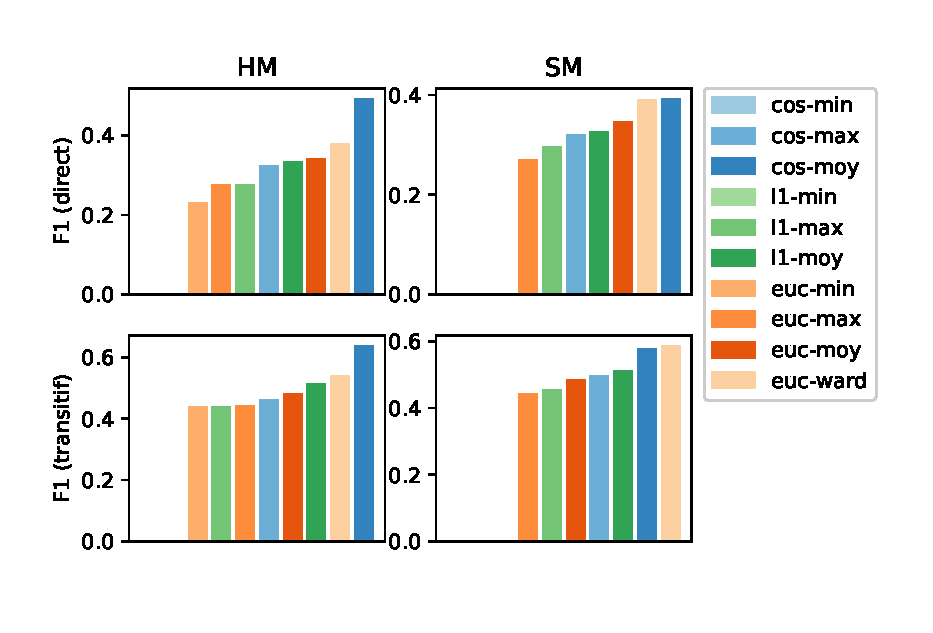
\includegraphics[width=0.7\textwidth]{fig/plot/taxex_cluparams-all.eps}
    \caption[Influence des paramètres de regroupement sur l'extraction de taxonomie]{Mesures $F_1$ obtenues pour différentes combinaisons de distances (euclidienne, cosinus, $L_1$) et de critères de liaison (\textit{min} pour saut minimal, \textit{max} pour saut maximal, \textit{moy} pour saut moyen, \textit{ward} pour distance de Ward). Les scores sont moyennés sur tous les modèles de plongement, et calculés selon l'évaluation directe (\textit{en haut}) et transitive (\textit{en bas}), pour les deux variantes Hard Mapping (HM, \textit{à gauche}) et Soft Mapping (SM, \textit{à droite}).}
    \label{fig:taxex-cluparams-all}
\end{figure}

\subsection{Base du softmax et seuil de probabilité}
\label{subsec:te-hp-softmapping}

Les deux autres hyperparamètres sont propres à la méthode Soft Mapping : il s'agit de la base $\beta$ du softmax, et du seuil de probabilité $t$. La base du softmax contrôle le piqué des distributions de probabilité $P(Z_t = C)$ autour des clusters qui ont la plus forte mesure $F_1$ : une valeur élevée concentre l'essentiel de la masse de probabilité sur le meilleur cluster, tandis qu'une valeur nulle distribue cette masse à tous les clusters. Le seuil de probabilité $t$ est utilisé pour filtrer la liste d'axiomes de subsumption lors de l'étape de reconstruction taxonomique : seuls les axiomes $(B \sqsubset A)$ qui vérifient $P(B \sqsubset A) > t$ sont conservés et ajoutés au graphe acyclique $G$. Dans toute la suite, le modèle de plongement utilisé est TransE et le regroupement se fait avec la distance cosinus et le critère du saut moyen, puisque ce sont les paramètres qui donnent le meilleur $F_1$ sur toutes les évaluations. 

Un jeu d'évaluation $X$ est constitué d'un jeu de données d'entrée $\cal{D}$, contenant des plongements vectoriels et les types correspondants, et d'une taxonomie de référence $T^*$. Pour des paramètres fixés, on peut extraire une taxonomie $\hat{T}$ à partir de $\cal{D}$, comparer cette taxonomie à la référencec $T^*$, et calculer les métriques précédentes : précision $p$, rappel $r$ et $F_1$, de façon directe, transitive ou moyenne. 

Pour un jeu d'évaluation $X$, on choisit comme métrique d'évaluation la mesure $F_1$ moyenne : c'est la mesure la plus synthétique, puisque le $F_1$ est une moyenne de la précision et du rappel, et que le $F_1$ moyen est lui-même la moyenne du $F_1$ direct et du $F_1$ transitif; on le note $F_1^M(X, \beta, t)$ pour mettre en évidence la dépendance en les paramètres $t$ et $\beta$, ainsi qu'en les données d'évaluation $X$.
On peut alors chercher les valeurs optimales des paramètres :
\begin{equation}
  \beta^*(X), t^*(X) = \argmax_{\substack{t \in [0, 1] \\ \beta \in \R_+}} F_1^M(X, \beta, t)
\end{equation}
Ces paramètres optimaux peuvent par exemple être estimés avec une \textit{grid search} : on discrétise l'espace de recherche, ce qui nous donne un nombre fini de combinaisons de paramètres possibles, et on évalue l'algorithme sur chacune de ces combinaisons. Par exemple, $t$ varie dans $[0, 1]$ et $\beta$ dans $\R_+$ : on peut diviser le premier intervalle en $\{0, 0.25, 0.5, 0.75, 1\}$ et le second en $\{0, 100, 500, 1000 \}$, soit cinq valeurs possibles pour $t$ et quatre pour $\beta$, donc vingt combinaisons à essayer au total. Cette recherche peut être améliorée en tirant aléatoirement des couples de $[0, 1] \times \R_+$, ce qui permet généralement de mieux couvrir l'espace de recherche \cite{bergstra2012random}.

En pratique, on veut pouvoir appliquer notre approche sur des données d'entrée pour lesquelles on ne dispose pas de taxonomie de référence, puisque le but est précisément d'extraire une telle taxonomie. C'est un problème non-supervisé, on ne peut donc pas utiliser de validation croisée.
De plus, les valeurs de $\beta^*$ et $t^*$ optimales calculées pour un certain jeu de données ne sont \textit{a priori} pas optimales pour un autre jeu de données. 
Plutôt que calculer $\beta^*$ et $t^*$, on souhaite plutôt trouver des valeurs «raisonnables» de $\beta$ et de $t$, autrement dit des valeurs permettant, en moyenne, de ne pas trop s'éloigner de l'optimum.

Pour cela, on définit un ensemble de jeux d'évaluation de référence $\cal{X} = (X_1, X_2, \ldots, X_r)$, et on cherche une valeur de $t$ et de $\beta$ qui permettent d'approcher le score $F_1$ optimal sur chacun des $X_k$ :
\begin{equation}
    \hat{\beta}, \hat{t} = \argmax_{\substack{t \in [0, 1] \\ \beta \in \R_+}} \frac{1}{| \cal{X} |} \sum_{X \in \cal{X}} \frac{\displaystyle F_1^M(X, \beta, t)}{\displaystyle F_1^M(X, \beta^*(X), t^*(X))}
\end{equation}

Le quotient $\frac{ F_1^M(X, \beta, t)}{ F_1^M(X, \beta^*(X), t^*(X))}$ permet d'exprimer les performances du modèle pour $t$ et $\beta$ comme une fraction des performances optimales – en effet, l'enjeu ici n'est pas les performances absolues du modèle, mais l'écart entre les performances maximales possibles et les performances atteintes avec $\beta$ et $t$. On appelle cette quantité le \textit{score} associé aux paramètres $\beta$ et $t$, qui varie entre 0 et 1 :
\begin{equation}
    S(\beta, t; X) = \frac{\displaystyle F_1^M(X, \beta, t)}{\displaystyle F_1^M(X, \beta^*(X), t^*(X))}
\end{equation}
%
Et l'on cherche à maximiser le score moyen associé à un couple de paramètres :
\begin{equation}
    \bar{S}(\beta, t) = \frac{1}{| \cal{X} |} \sum_{X \in \cal{X}} S(\beta, t; X)
\end{equation}


Alternativement, on pourrait choisir de maximiser le pire des scores, plutôt que la moyenne des scores. Le score minimal d'un couple de paramètres est le pire score obtenu sur l'ensemble des jeux de référence :
\begin{equation}
    S_{\min}(\beta, t) = \min_{X \in \cal{X}} S(\beta, t; X)
\end{equation}
En comparaison du score moyen, maximiser le score minimal permet de se prémunir contre des valeurs de paramètres qui fonctionnent bien dans le cas général mais donnent de très mauvais résultats dans certains cas :
\begin{equation}
    \hat{\beta}, \hat{t} = \argmax_{\substack{t \in [0, 1] \\ \beta \in \R_+}}
    S_{\min}(\beta, t)
\end{equation}


L'enjeu des paragraphes suivants est double : d'une part, trouver des valeurs satisfaisantes pour $\hat{\beta}$ et $\hat{t}$, et d'autre part, comprendre l'effet de $\beta$ et de $t$ sur la taxonomie extraite.

\subsubsection{Choix de \texorpdfstring{$\beta$}{beta} et \texorpdfstring{$t$}{t}}
\label{subsec:te-hp-values}

Pour trouver $\hat{\beta}$ et $\hat{t}$, on construit aléatoirement cinq sous-taxonomies de DBpédia de différentes tailles et de différentes profondeurs, afin de constituer l'ensemble $\cal{X}$.
On applique alors notre méthode d'extraction de taxonomie à ces cinq sous-taxonomies pour vingt valeurs de $\beta$ réparties linéairement dans l'intervalle $[1, 200]$. Pour chacune des valeurs de $\beta$, on fait varier $t$ dans l'intervalle $[0, 1]$ (à nouveau en séparant l'intervalle en vingt valeurs espacées linéairement), ce qui nous permet d'obtenir empiriquement le seuil optimal $t^*(\beta)$. On obtient ainsi un tableau reliant chaque couple de paramètres $(\beta, t) \in [0, 200] \times [0, 1]$  et chaque sous-taxonomie $X_k$ au score associé $S(\beta, t; X_k)$.


\begin{figure}[h]
    \centering
    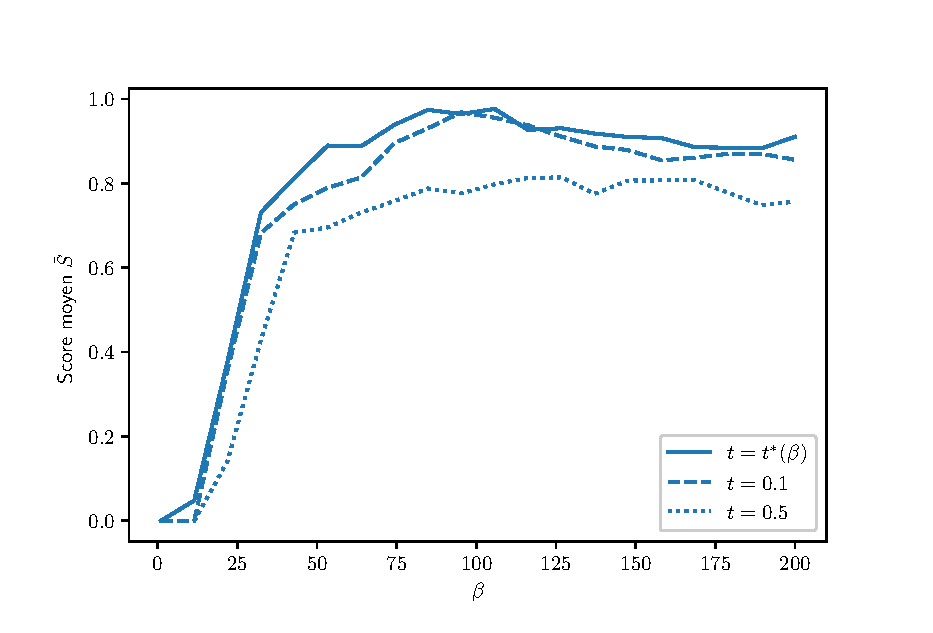
\includegraphics[width=0.7\textwidth]{fig/plot/average_beta_vs_best_all_FR.eps}
    \caption[Influence du paramètre $\beta$]{Résultats de l'extraction de taxonomie pour différentes valeurs du paramètre $\beta$, pour le seuil optimal $t^*(\beta)$ et pour deux seuils fixes $t=0.1$ et $t=0.5$. 
    L'ordonnée représente le score moyen $\bar{S}(\beta, t)$, qui est la moyenne des mesures $F_1^M$ sur les cinq sous-taxonomies de $\cal{X}$, exprimées comme une fraction de l'optimum.
    %L'ordonnée représente la moyenne des mesures $F_1$ obtenues par évaluation directe et transitive sur cinq sous-taxonomies de DBpédia, exprimée comme une fraction de l'optimum.
    }
    \label{fig:beta-search-1}
\end{figure}

On trace alors les résultats obtenus, pour trois valeurs de $t$ : deux valeurs fixes, $t = 0.1$ et $t = 0.5$, et la valeur optimale $t = t^*(\beta)$ qui indique le meilleur score que l'on puisse espérer atteindre. Le résultat est présenté dans la figure \ref{fig:beta-search-1}. Pour les trois valeurs de $t$, on observe le comportement suivant : la mesure $F_1$ moyenne est nulle pour $\beta = 1$, augmente abruptement, atteint un maximum autour de $\beta = 100$, puis diminue progressivement. 

\begin{figure}
    \centering
    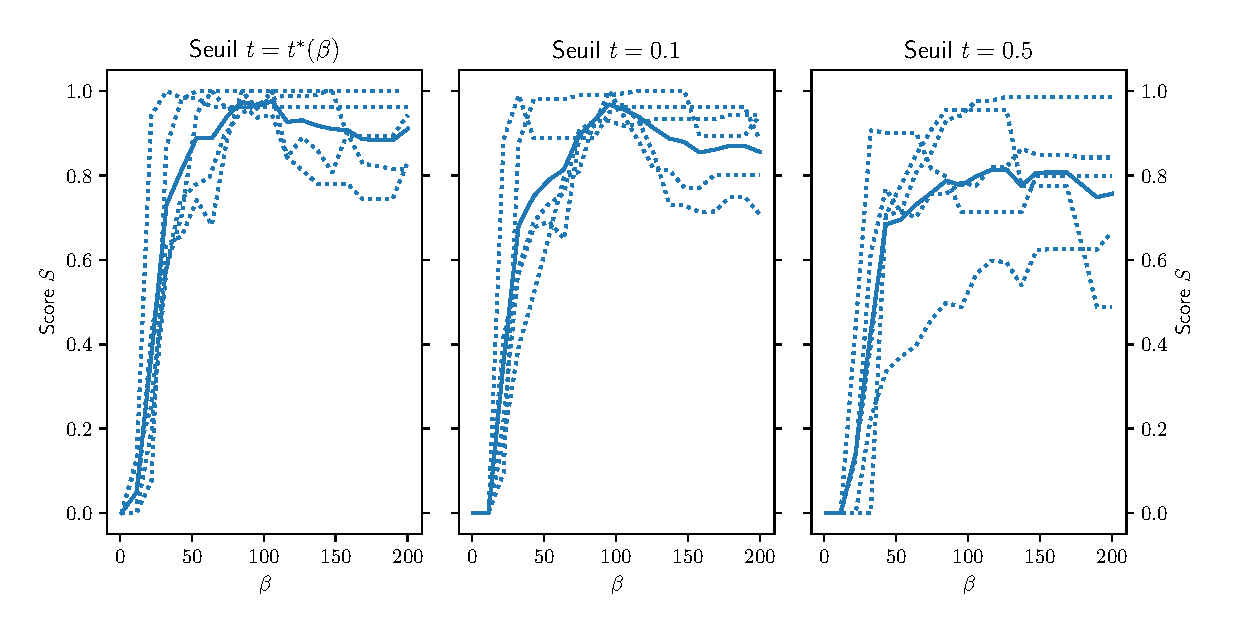
\includegraphics[width=\textwidth]{fig/plot/average_beta_breakdown_all3_FR.eps}
    \caption[Scores selon $\beta$ sur cinq sous-taxonomies]{Scores obtenus pour différentes valeurs de $\beta$ dans l'intervalle $[0, 200]$, pour le seuil optimal $t^*(\beta)$ (\textit{à gauche}), et pour deux seuils fixes 0.1 et 0.5. Chaque ligne pointillée représente les résultats pour une sous-taxonomie $X_i$; la ligne continue représente la moyenne sur les cinq sous-taxonomies.}
    \label{fig:beta-search-3}
\end{figure}

Pour mieux comprendre les variabilités de $S$ d'un jeu de données à l'autre, on affiche la courbe des scores en fonction de $\beta$ pour chacune des cinq sous-taxonomies. Le résultat est présenté dans la figure \ref{fig:beta-search-3}. On observe des disparités importantes d'une taxonomie à l'autre, pour les trois valeurs de $t$. 

Dans le cas $t=t^*$, le score maximal est obtenu dès $\beta = 50$ pour l'une des taxonomies, et pour $\beta = 150$ pour une autre. Dans certains cas, les résultats diminuent sitôt le maximum atteint; dans d'autres, on observe au contraire un long plateau. Toutefois, pour toutes les taxonomies, le score atteignable en $\beta=100$ est proche du score maximal, c'est-à-dire que $S(\beta=100, t=t^*(\beta);X_i)$ est proche de $S(\beta^*, t^*; X_i)$ pour tous les $X_i \in \cal{X}$. Cela donne un score moyen $\bar{S}(\beta=100, t=t^*(\beta))$ égal à $97,7\%$, et un score minimal $S_{\min}(\beta, t)$ égal à $94,4\%$.

Pour $t=0.1$, le comportement est globalement le même que dans le cas précédent. À nouveau, on observe d'une part des disparités de comportement entre les taxonomies, et d'autre part un rapprochement des courbes autour de $\beta=100$; choisir cette valeur de $\beta$ conduit à un score moyen de $96.9\%$ et à un score minimal de $92.9\%$. Dans les deux cas $t=t^*$ et $t=0.1$, prendre comme critère le score moyen ou le score minimal est indifférent : la valeur de $\beta$ qui maximise l'un est également celle qui maximise l'autre.

Le cas $t=0.5$ est différent. Une nouvelle fois, on observe une augmentation abrupte du score dans l'intervalle $[0, 50]$, mais les disparités entre taxonomies sont fortement accrues. De plus, les scores sont significativement inférieurs au cas précédent; le score ne dépasse pas $90\%$ sur trois des cinq taxonomies. Enfin, les scores maximaux pour chaque taxonomie sont atteints en des points éloignés, ce qui grève le score moyen. Ce dernier atteint un maximum en $\beta=125$ et vaut alors $81.4\%$; le score minimal, lui, atteint son maximum en $\beta=150$ et vaut alors $62.5\%$.

\begin{figure}[h]
    \centering
    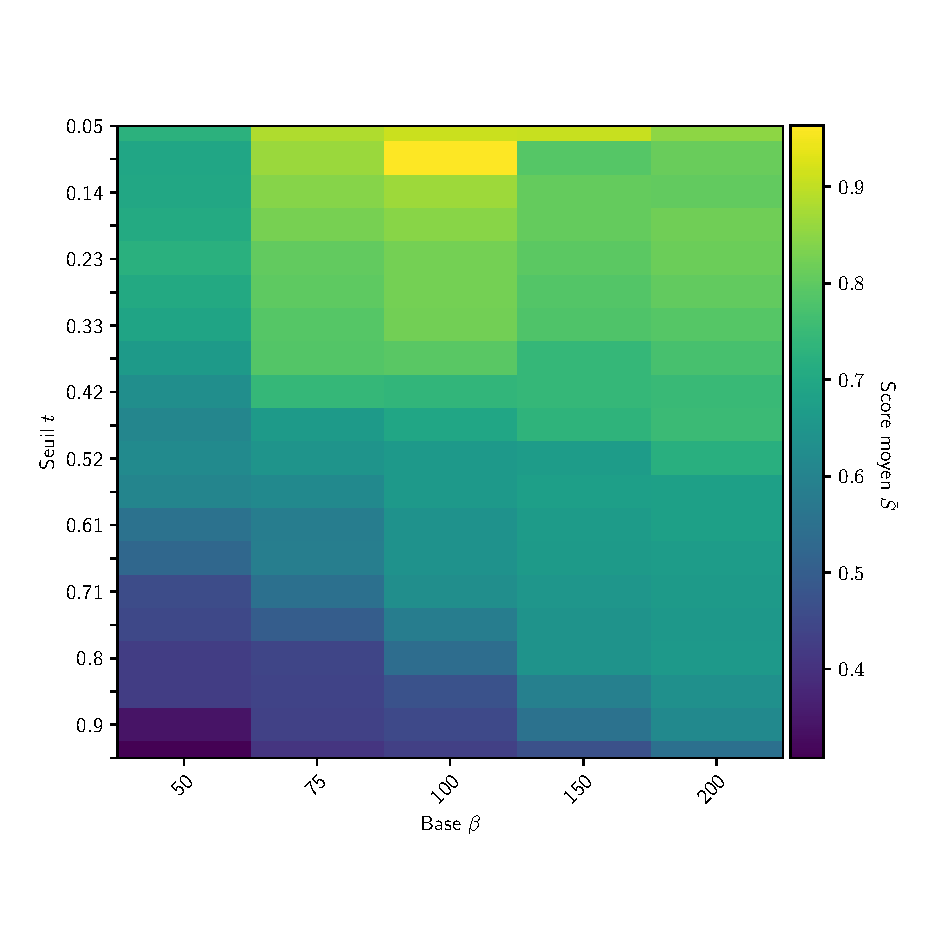
\includegraphics[width=0.7\textwidth]{fig/tb_heatmap.eps}
    \caption[Scores d'extraction moyens, pour différents $\beta$ et $t$]{Scores moyens obtenus sur cinq sous-taxonomies pour différentes valeurs de $\beta$ et de $t$.}
    \label{fig:betea-search-4}
\end{figure}

Finalement, pour explorer d'autres valeurs du seuil $t$, on affiche directement le score moyen $\bar{S}(\beta, t)$ pour vingt valeurs de $t$ dans $[0, 20]$ et pour $\beta \in \{50, 75, 100, 150, 200\}$. Les résultats sont affichés à la figure \ref{fig:betea-search-4}. À nouveau, les meilleurs résultats sont observés pour $\beta = 75$ ou $\beta=100$ et pour des seuils faibles. On observe un maximum du score moyen $\bar{S}$ pour les valeurs $\beta = 100, t = 0.1$. De toutes ces observations, on utilisera par défaut les valeurs $\hat{\beta} = 100$ et $\hat{t} = 0.1$.

Cependant, cette recherche d'hyperparamètres demeure très limitée. D'une part, on s'est restreint aux plongements TransE avec distance cosinus et critère du saut moyen : d'autres modèles de plongement ou d'autres paramètres de regroupement pourraient conduire à d'autres valeurs de $\hat{\beta}$ et $\hat{t}$. De plus, les cinq sous-taxonomies de référence sont toutes issues de DBpédia, et ne représentent pas nécessairement l'ensemble des graphes de connaissance. Aussi, les valeurs données ici ne doivent pas être considérées comme des choix définitifs.

% Dans les deux sections suivantes, on cherche à mieux comprendre l'effet de $\beta$ et de $t$ sur les taxonomies suivantes
% Ces observations concordent avec l'analyse qualitative : il est nécessaire de fixer une valeur de $\beta$ suffisamment élevée pour séparer suffisamment les axiomes vrais des axiomes faux. Pour $\beta$ suffisamment élevé en revanche, on observe une relative stabilisation du score, plus ou moins marquée selon $t$. 
% Enfin, en fixant $\beta = 100$ et $t=0.1$, on obtient une mesure $F_1$ moyenne supérieure à 95\% de la mesure $F_1$ optimale. C'est donc ces valeurs des paramètres que l'on utilisera par défaut, et qui ont servi pour les résultats présentés à la section précédente.


\subsubsection{Influence de \texorpdfstring{$\beta$}{beta}}
\label{subsec:te-hp-beta}

Pour observer qualitativement l'effet de $\beta$ sur les probabilités des axiomes de subsumption, on affiche les superclasses les plus probables de quelques classes choisies : \dbo{Athlete}, \dbo{Song}, \dbo{Event} (en français : Athlète, Chanson, Événément). Par superclasse la plus probable d'une classe $x$, on entend la classe $y$ telle que la probabilité $P(x \sqsubset y)$ soit supérieure à toutes les autres probabilités $P(x \sqsubset y')$. Le résultat est affiché dans le tableau \ref{tab:hp-most-prob-axioms}. Dans la taxonomie de référence, \dbo{Athlete} et \dbo{Song} ont deux superclasses (\dbo{Person}, \dbo{Agent} et \dbo{MusicalWork}, \dbo{Work} respectivement), tandis que \dbo{Event} n'en a aucune.


\begin{table}[h]
    \centering
    \caption[Prédiction de superclasses pour différentes valeurs de $\beta$]{Les trois superclasses les plus probables de \dbo{Athlete} (\textit{en haut}), de \dbo{Song} (\textit{au milieu}), et de \dbo{Event} (\textit{en bas}), avec les probabilités $p$ associées, pour différentes valeurs de $\beta$ entre $1$ et $100$ (une ligne pour chaque valeur de $\beta$, les préfixes \dbo{} sont omis par souci de concision).}

\begin{tabular}{|l|cr|cr|cr|}
\hline
& \multicolumn{2}{c|}{1} & \multicolumn{2}{c|}{2} & \multicolumn{2}{c|}{3} \\
$\beta$	&	classe	&	$p$	&	classe	&	$p$	&	classe	&	$p$  \\ 
\hline
1 & Agent & 0.00 & Event & 0.00 & Species & 0.00 \\5 & Event & 0.00 & Agent & 0.00 & Species & 0.00 \\10 & Event & 0.02 & SportsSeason & 0.01 & Document & 0.01 \\30 & Agent & 0.97 & Person & 0.00 & Species & 0.00 \\50 & Agent & 1.00 & Person & 0.02 & Organisation & 0.00 \\100 & Agent & 1.00 & Person & 0.41 & Organisation & 0.00 \\
\hline
\end{tabular}

\vspace{2mm}

\begin{tabular}{|l|cr|cr|cr|}
\hline
& \multicolumn{2}{c|}{1} & \multicolumn{2}{c|}{2} & \multicolumn{2}{c|}{3} \\
$\beta$	&	classe	&	$p$	&	classe	&	$p$	&	classe	&	$p$  \\ 
\hline
1 & Agent & 0.00 & Event & 0.00 & Species & 0.00 \\5 & Event & 0.00 & Agent & 0.00 & Species & 0.00 \\10 & Event & 0.02 & SportsSeason & 0.01 & Document & 0.01 \\30 & Agent & 0.25 & MusicalWork & 0.12 & Species & 0.06 \\50 & Work & 0.87 & MusicalWork & 0.67 & Single & 0.20 \\100 & Work & 1.00 & MusicalWork & 0.81 & Single & 0.14 \\
\hline
\end{tabular}

\vspace{2mm}

\begin{tabular}{|l|cr|cr|cr|}
\hline
& \multicolumn{2}{c|}{1} & \multicolumn{2}{c|}{2} & \multicolumn{2}{c|}{3} \\
$\beta$	&	classe	&	$p$	&	classe	&	$p$	&	classe	&	$p$  \\ 
\hline
1 & Agent & 0.00 & Species & 0.00 & Place & 0.00 \\5 & Agent & 0.00 & Species & 0.00 & Document & 0.00 \\10 & SportsSeason & 0.01 & Document & 0.00 & Agent & 0.00 \\30 & Work & 0.00 & Eukaryote & 0.00 & Place & 0.00 \\50 & Work & 0.00 & Place & 0.00 & ArchitecturalStructure & 0.00 \\100 & Person & 0.00 & Organisation & 0.00 & ArchitecturalStructure & 0.00 \\
\hline
\end{tabular}

    \label{tab:hp-most-prob-axioms}
\end{table}



Étudions d'abord les deux premiers tableaux. Dans les deux cas, on observe des résultats incohérents pour $\beta < 30$ : d'une part, les superclasses les plus probables ne correspondent pas aux vraies superclasses; d'autre part, les probabilités de toutes les superclasses sont très proches de zéro, ce qui ne permet pas de distinguer les axiomes pertinents des autres. Lorsque $\beta$ augmente (ici $\beta = 30$), les vraies superclasses commencent à émerger. Pour \dbo{Athlete}, les deux superclasses les plus probables sont bien les vraies superclasses; l'une d'elle  (\dbo{Agent}) est prédite avec probabilité 0.97, ce qui est satisfaisant; en revanche, l'autre (\dbo{Person}) est prédite avec une probabilité très faible. Il faut attendre $\beta = 100$ pour discriminer nettement les classes valides (\dbo{Agent} et \dbo{Person}, prédites avec probabilités $1$ et $0.41$ respectivement) des classes invalides (\dbo{Organisation}, avec probabilité $0.0$). Les mêmes observations s'appliquent à \dbo{Song} : les vraies superclasses émergent et se détachent progressivement des fausses superclasses. Dans ce cas, on note aussi que \dbo{Single}, qui n'est pas une superclasse de \dbo{Song} mais une classe sémantiquement proche, se voit attribuer une probabilité relativement élevée (entre $0.1$ et $0.2$).

Enfin, dans le cas de \dbo{Event}, le modèle prédit correctement des probabilités nulles pour tous les axiomes de subsumption possibles, et ce, quelle que soit la valeur de $\beta$. Cela correspond bien à la réalité, puisque \dbo{Event} ne possède aucune superclasse.

Si l'on examine maintenant les taxonomies extraites pour différentes valeurs de $\beta$, on obtient la figure \ref{fig:hp-beta-taxonomies} (seules quelques classes sont représentées, pour faciliter l'affichage). Comme prévu, le cas $\beta = 1$ n'aboutit à rien : on obtient un arbre dégénéré. Quand $\beta$ augmente, les deux classes de niveau 1 (\dbo{Place} et \dbo{Agent}) sont identifiées, mais l'une est incorrectement considérée comme sous-classe de l'autre. Aucune hiérarchie ne se distingue sur les autres classes. Puis, pour $\beta=50$, les deux classes principales sont correctement séparées, et leurs sous-classes attribuées sans erreur. Une hiérarchie commence à se dessiner dans les sous-classes de \dbo{Place}, avec d'un côté les lieux habités (\dbo{PopulatedPlace} et \dbo{Region}), et de l'autre les espaces naturels (\dbo{NaturalPlace}, \dbo{Mountain}, \dbo{Volcano}). Enfin, pour $\beta=100$, la taxonomie est correctement extraite, avec une seule erreur (\dbo{Volcano} n'est pas sous-classe de \dbo{Mountain} dans la taxonomie de référence, même si cette classification aurait une certaine logique). Ces observations illustrent comment l'émergence progressive des superclasses quand $\beta$ augmente, décrite dans les paragraphes précédents, se traduit par une structuration croissante de la taxonomie extraite.

\begin{figure}[h]
    \centering
    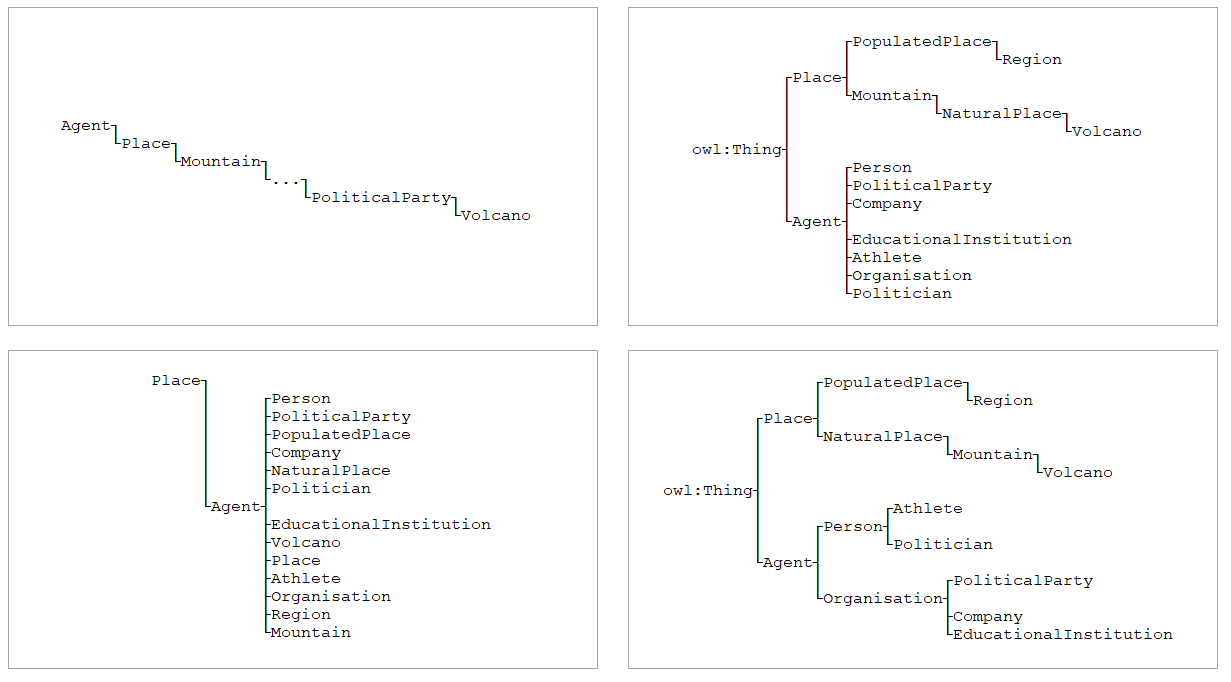
\includegraphics[width=\textwidth]{img/tax_samples.png}
    \caption[Exemples de taxonomies partielles pour différentes valeurs de $\beta$]{Exemples de taxonomies partielles pour $\beta = 1$ (\textit{en haut à gauche}), $\beta = 15$ (\textit{en bas à gauche}), $\beta=50$ (\textit{en haut à droite}) et $\beta=100$ (\textit{en bas à droite}). \small Note: la classe \texttt{owl:Thing} n'est pas présente dans les données, elle est ajoutée automatiquement lorsqu'il y a plus d'une classe sans parents dans la taxonomie extraite.}
    \label{fig:hp-beta-taxonomies}
\end{figure}


% de \dbo{Mountain}, c'est-à-dire les classes $x$ telles que  $P(\dbo{Mountain} \sqsubset x)$ soit maximales. Le résultat est affiché dans le tableau \ref{tab:hp-most-prob-axioms}. Dans la taxonomie DBpédia, \dbo{Mountain} a deux superclasses, \texttt{Place} et \texttt{NaturalPlace}. On observe ici que les résultats sont incohérents pour $\beta \leq 20$ : tous les axiomes ont des probabilités très faibles, inférieures à $0,02$. Quand $\beta$ augmente (cas $\beta = 30$), les superclasses correctes émergent, mais leurs probabilités sont encore faibles. Puis, pour $\beta \geq 50$, ces deux superclasses se distinguent nettement des autres, allant jusqu'à atteindre des probabilités de $0,93$ et $0,83$ respectivement, tandis que les probabilités des autres classes ne dépassent pas $0,01$. Enfin, on observe que l'axiome $\texttt{Mountain} \sqsubset \texttt{Place}$ a une plus grande probabilité que $\texttt{Mountain} \sqsubset \texttt{NaturalPlace}$, ce qui correspond à l'intuition. % TODO: expliquer pourquoi?



\subsubsection{Seuil de probabilité}
\label{subsec:te-hp-threshold}



\begin{figure}[h]
    \centering
    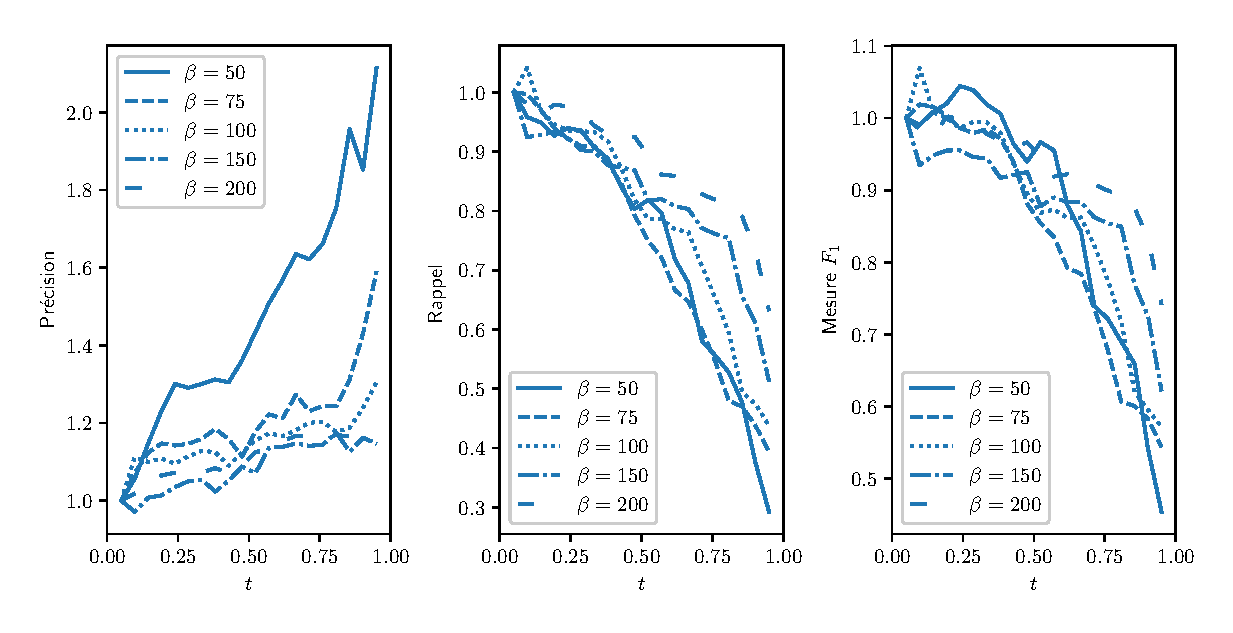
\includegraphics[width=\textwidth]{fig/plot/threshold_breakdown_aggregated.eps}
    \caption[Influence du seuil de probabilité sur l'extraction de taxonomie pour différents $\beta$]{Précision, rappel et mesure $F_1$ moyens, pour différentes valeurs du seuil $t$ et différentes valeurs de $\beta$. Pour faciliter la comparaison des tendances, les résultats sont normalisés de façon à avoir chaque ligne commençant à 1 en $t = 0$.}
    \label{fig:threshold-search-2}
\end{figure}

Pour comprendre l'effet du seuil $t$, on s'intéresse à l'évolution de la précision, du rappel et du $F_1$ lorsque $t$ varie entre $0$ et $1$, pour différentes valeurs de $\beta$. On calcule la moyenne de ces trois métriques sur les cinq sous-taxonomies utilisées précédemment. Les résultats sont affichés dans la figure \ref{fig:threshold-search-2}.

En moyenne, on observe les effets suivants : la précision augmente avec $t$, tandis que le rappel diminue. Ces deux effets étaient attendus : en augmentant le seuil, on élimine les axiomes les plus incertains, c'est-à-dire ceux qui ont le plus de chance d'être faux. La précision, autrement dit la proportion d'axiomes extraits qui sont vrais, augmente donc. Mais, parmi les axiomes éliminés par l'augmentation du seuil, certains étaient vrais : la proportion d'axiomes vrais qui sont effectivement extraits, c'est-à-dire le rappel, diminue.

Ces tendances sont plus ou moins marquées selon $\beta$ : la précision augmente d'autant plus avec $t$ que $\beta$ est faible; de même, la diminution du rappel avec $t$ semble plus rapide pour les valeurs faibles de $\beta$. Selon les valeurs de $\beta$, ces deux tendances (augmentation de la précision et diminution du rappel) se compensent plus ou moins tant que $t$ est faible. Dans les cinq cas, le $F_1$ observé sur l'intervalle $t \in [0, 0.4]$ est proche du $F_1$ maximal ($10\%$ d'écart au maximum). Toutefois, passé un certain seuil proche de $t=0.5$, l'augmentation de la précision ne suffit plus à compenser la diminution du rappel et la mesure $F_1$ chute alors, quelle que soit la valeur de $\beta$.

% on fixe $\beta = 100$, et pour différentes valeurs de $t$ dans l'intervalle $[0, 1]$, on évalue la méthode d'extraction sur chacune des cinq sous-taxonomies selon les métriques présentées dans la section précédente : moyennes de la précision, du rappel et de la mesure $F_1$ pour l'évaluation directe et transitive.
%
% Les résultats sont représentés dans la figure \ref{fig:threshold-search-1}. % : chaque ligne pointillée représente les résultats pour l'une des taxonomies, tandis que la ligne pleine est la moyenne des résultats sur les cinq taxonomies. Pour faciliter la comparaison des tendances, les résultats sont normalisés de façon à avoir $y=1$ pour $t = 0$.
%
%En moyenne, on observe les effets suivants : la précision augmente avec $t$, tandis que le rappel diminue. Ces deux effets étaient attendus : en augmentant le seuil, on élimine les axiomes les plus incertains, c'est-à-dire ceux qui ont le plus de chance d'être faux. La précision, autrement dit la proportion d'axiomes extraits qui sont vrais, augmente donc. Mais, parmi les axiomes éliminés par l'augmentation du seuil, certains étaient vrais : la proportion d'axiomes vrais qui sont effectivement extraits, c'est-à-dire le rappel, diminue.
%
%De plus, l'augmentation de la précision est insuffisante pour compenser la diminution du rappel, ce qui implique que la mesure $F_1$ diminue également avec $t$. 

\begin{figure}[h]
    \centering
    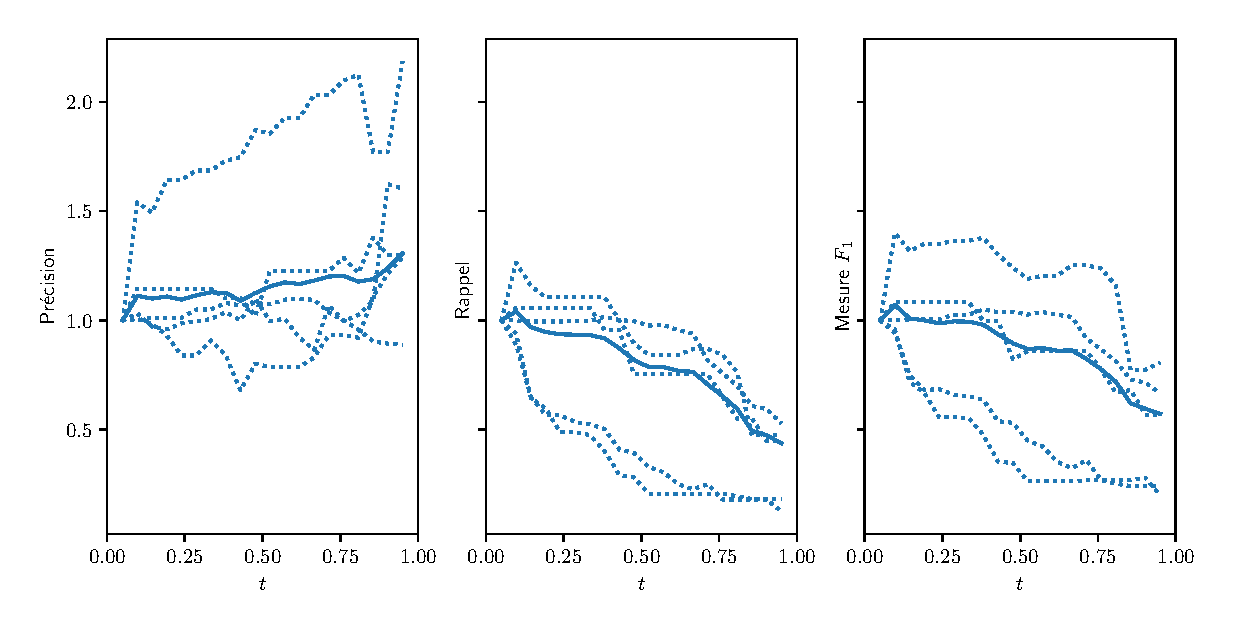
\includegraphics[width=\textwidth]{fig/plot/threshold_breakdown_avg_no_event.eps}
    \caption[Influence du seuil de probabilité sur l'extraction de taxonomie pour $\beta=100$]{Précision, rappel et mesure $F_1$ mesurés sur cinq sous-taxonomies, pour différentes valeurs du seuil $t$ et pour $\beta=100$. Chaque ligne pointillée représente les résultats pour l'une des taxonomies, tandis que la ligne pleine est la moyenne des résultats sur les cinq taxonomies. Pour faciliter la comparaison des tendances, les résultats sont normalisés de façon à avoir chaque ligne commençant à 1 en $t = 0$.}
    \label{fig:threshold-search-1}
\end{figure}

Pour affiner ces observations, on fixe $\beta = 100$, et on affiche le détail des résultats pour chacune des cinq taxonomies $X_i$ dans la figure \ref{fig:threshold-search-1}. On observe également une grande hétérogénéité d'une taxonomie à l'autre. En particulier, l'augmentation de la précision avec $t$ est très nette pour l'un des modèles, mais moins pour les autres. De plus, la diminution du rappel est très rapide (dès $t > 0.05$) pour deux des modèles; pour les cinq autre, le rappel est assez stable dans l'intervale $[0, 0.5]$, et diminue ensuite. Cette hétérogénéité s'observe aussi pour la mesure $F_1$ : dans un cas, elle est stable dans l'intervalle $[0.1, 0.7]$ et diminue ensuite régulièrement; dans deux autres cas, elle est stable sur $[0.1, 0.5]$, diminue vers un plateau sur $[0.5, 0.75]$, et diminue encore après $0.75$; dans les deux derniers cas, elle diminue rapidement dès que $t$ s'écarte de $0$.

% Cette hétérogénéité des comportements rend difficile le choix définitif d'une valeur pour $t$; toutefois, choisir une valeur basse telle que $t = 0.1$ paraît donner les meilleurs résultats en moyenne.

%Les résultats sont représentés dans la figure \ref{fig:beta-search-2}. Pour l'évaluation transitive, on observe que la précision augmente avec $t$, tandis que le rappel diminue. Cette conclusion était attendue : en augmentant le seuil, on élimine les axiomes les plus incertains, c'est-à-dire ceux qui ont le plus de chance d'être faux. La précision, autrement dit la proportion d'axiomes extraits qui sont vrais, augmente donc. Mais, parmi les axiomes éliminés par l'augmentation du seuil, certains étaient vrais : la proportion d'axiomes vrais qui sont effectivement extraits, c'est-à-dire le rappel, diminue. Ces deux effets, augmentation de la précision et diminution du rappel avec $t$, se compensent globalement dans l'intervalle $[0.1, 0.7]$, comme le montre la courbe du $F_1$. Au-delà de $0.7$, l'augmentation de la précision n'est plus suffisante pour compenser la chute du rappel. En effet, pour $t > 0.7$, plus de 95\% des axiomes extraits sont vrais : en augmentant le seuil, on élimine mécaniquement un grand nombre d'axiomes vrais, d'où la chute du rappel et donc de la mesure $F_1$.


